\documentclass{problemset}
\usepackage{amsmath}

\usepackage{lipsum}
%\usepackage{showframe}
%\usepackage{layout}


%\usepackage{geometry}
%\geometry{textwidth=5.5in, hoffset=-0.5in, voffset=0in, textheight=10in, footskip=20pt, 
%marginparsep=10pt,
%marginparwidth=1.75in,
%%showframe
%}
\usepackage[charter,cal=cmcal]{mathdesign} %different font
\usepackage{microtype}
\usepackage{amsmath}
%\usepackage{amsfonts}
%\usepackage{amssymb}
\usepackage{graphicx}
\usepackage[inline]{enumitem}
\usepackage{xparse}
\usepackage{ifthen}
\usepackage{graphicx}
\usepackage{caption}
\usepackage{subcaption}
\usepackage{color}
\usepackage{tikz}
\usepackage{fancyhdr}
\usepackage{calc}
\usepackage{wrapfig}
\usepackage{marginnote}
\usepackage{mparhack}
\usepackage{marginfix}
\usepackage[hidelinks]{hyperref}


\usepackage{pgfplots}
\pgfplotsset{compat=newest}
%%%
% Useful Linear Algebra macros
%%%
\newcommand{\ul}{$\underline{\phantom{xxx}}$}
\newcommand{\ull}{\underline{\phantom{xxx}}}
\newcommand{\xh}{{\hat {\mathbf x}}}
\newcommand{\yh}{{\hat {\mathbf y}}}
\newcommand{\zh}{{\hat {\mathbf z}}}
\newcommand{\R}{\mathbb{R}}
\newcommand{\Z}{\mathbb{Z}}
\newcommand{\N}{\mathbb{N}}
\newcommand{\proj}{\mathrm{proj}}
\newcommand{\Proj}{\mathrm{proj}}
\newcommand{\Comp}{\mathrm{comp}}
\newcommand{\Perp}{\mathrm{perp}}
\renewcommand{\span}{\mathrm{span}\,}
\newcommand{\Span}{\mathrm{span}\,}
\newcommand{\Img}{\mathrm{img}\,}
\newcommand{\Null}{\mathrm{null}\,}
\newcommand{\Range}{\mathrm{range}\,}
\newcommand{\rref}{\mathrm{rref}}
\newcommand{\rank}{\mathrm{rank}}
\newcommand{\Rank}{\mathrm{rank}}
\newcommand{\nnul}{\mathrm{nullity}}
\newcommand{\mat}[1]{\begin{bmatrix}#1\end{bmatrix}}
\newcommand{\chr}{\mathrm{char}}
\renewcommand{\d}{\mathrm{d}}

%\tcbuselibrary{skins}
%\usetikzlibrary{shadings}


%%%
% Set up the margins to use a fairly large area of the page
%%%
%\textwidth=5.2in
%\topmargin=-1in
%\textheight=10in
%\parskip=.07in
%\parindent=0in


\fancypagestyle{siefken}{%
	\rfoot{\footnotesize\it \copyright\,Jason Siefken, 2015--2018 \ \makebox(30,5){
\includegraphics[height=1.2em]{by-sa.pdf}}}
	\lfoot{}
	\renewcommand{\headrulewidth}{0pt}
}
\fancypagestyle{iola}{%
	\rfoot{\footnotesize\it \copyright\,IOLA Team \url{iola.math.vt.edu} \ \makebox(30,5){
\includegraphics[height=2.2em]{images/iolalogo.png}}}
	\lfoot{}
	\renewcommand{\headrulewidth}{0pt}
}



\begin{document}
\pagestyle{empty}

\begin{center}
{\huge\bf Inquiry Based Linear Algebra}\\

\vspace{.7in}
{
\it \copyright\,Jason Siefken, 2016--2018 \\
Creative Commons By-Attribution Share-Alike\, \makebox(30,5){
\includegraphics[height=1.2em]{by-sa.pdf}}
}
\end{center}

\section*{About the Document}

	This document is a hybrid of many linear algebra resources, including those of
	the IOLA (Inquiry Oriented Linear Algebra) project, Jason Siefken's IBLLinearAlgebra
	project, and Asaki, Camfield, Moon, and Snipes' Radiograph and Tomography project.

	This document is a mix of student projects, problem sets, and labs.
	A typical class day looks like:
	\begin{enumerate}
		\item {\bf Introduction by instructor.} This may involve giving a definition,
			a broader context for the day's topics, or answering questions.
		\item {\bf Students work on problems.} Students work individually or in pairs
			on the prescribed problem.  During this time the instructor moves around
			the room addressing questions that students may have and giving one-on-one
			coaching.
		\item {\bf Instructor intervention.} If most students have successfully solved the 
			problem, the instructor regroups the class by providing a concise 
			explanation so that everyone is ready to move to the next concept.  This
			is also time for the instructor to ensure that everyone has understood the
			main point of the exercise (since it is sometimes easy to do some computation
			while being oblivious to the larger context).

			If students are having trouble, the instructor can give hints to the group,
			and additional guidance to ensure the students don't get frustrated
			to the point of giving up.
		\item {\bf Repeat step 2.}
	\end{enumerate}

	Using this format, students are working (and happily so) most of the class.
	Further, they are especially primed to hear the insights of the instructor, 
	having already invested substantially into each problem.

	This problem-set is geared towards concepts instead of computation, though some problems
	focus on simple computation.

	{\bf License}  Unless otherwise mentioned, pages of this document are licensed under the Creative Commons
	By-Attribution Share-Alike License.  That means, you are free to use,
	copy, and modify this document provided that you provide attribution
	to the previous copyright holders and you release your derivative work 
	under the same license.  Full text of the license is at \url{http://creativecommons.org/licenses/by-sa/4.0/}

	If you modify this document, you may add your name to the copyright list.  Also,
	if you think your contributions would be helpful to others, consider making a pull
	requestion, or opening an \emph{issue} at 
	\url{https://github.com/siefkenj/IBLLinearAlgebra}

	Content from other sources is reproduced here with permission and retains the Author's copyright.
	Please see the footnote of each page to verify the copyright.


\newpage


\addcontentsline{toc}{chapter}{Lessons}

\begin{lesson}
	\Title{Linear Combinations}

	\Heading{Textbook}
	Section 1.1

	\Heading{Objectives}
	\begin{itemize}
		\item Internalize vectors as geometric objects representing displacements.
		\item Use column vector notation to write vectors.
		\item Relate points an vectors and be able to interpret a point as a vector and a
			vector as a point.
		\item Solve simple equations involving vectors.
	\end{itemize}

	\Heading{Motivation}
	Students have differing levels of experience with vectors. We want to establish a common
	notation for vectors and use vector notation along with algebra to solve
	simple questions. E.g., ``How can I get to location $X$ given that I can only walk
	parallel to the lines $y=4x$ and $y=-x$?''

	\begin{annotation}
		\begin{notes}
			We will use the language
			\emph{component of $\vec v$ in the direction $\vec u$} in
			the future and it will be a \emph{vector}. For this reason, try
			to refer to the entries of a column vector as coordinates
			instead of components.
		\end{notes}
	\end{annotation}
	We will use column vector notation and the idea of equating coordinates in order to solve
	problems.

	\newpage
\end{lesson}


\setcounter{page}{1}
\pagestyle{iola}
\section*{Task 1.1: The Magic Carpet Ride}
\addcontentsline{toc}{subsection}{Task 1.1: The Magic Carpet Ride}

\begin{annotation}
	\begin{goals}
		\Goal{Hands-on experience with vectors as displacements.}
		\begin{itemize}
			\item Internalize vectors as geometric objects representing displacements.
			\item Use column vector notation to write vectors.
			\item Use pre-existing knowledge of algebra to answer vector
				questions.
		\end{itemize}
	\end{goals}
	\begin{notes}
		\begin{itemize}
			\item There are many ways to solve this problem,
				and some might start with equations. Make them
				draw a picture.
			\item When the students start coming up with
				vector equations, give them the vocabulary
				of \emph{linear combinations} and \emph{column
				vector notation}.
		\end{itemize}
	\end{notes}
\end{annotation}
You are a young traveler, leaving home for the first time. Your parents
want to help you on your journey, so just before your departure, they give
you two gifts. Specifically, they give you two forms of transportation:
a hover board and a magic carpet. Your parents inform you that both the
hover board and the magic carpet have restrictions in how they operate:


\begin{minipage}{\textwidth}
	\vspace{.5cm}
	\begin{wrapfigure}{l}{1in}
	\vspace{-.8cm}
	
\includegraphics[width=1in]{images/HoverBoard-small.png}
	\end{wrapfigure}

	We denote the restriction on the hover board's movement by the vector
	$\mat{3 \\1}$. By this we mean that if
	the hover board traveled ``forward'' for one hour, it would move along a
	``diagonal'' path that would result in a displacement of 3 miles East and
	1 mile North of its starting location.
\end{minipage}

\begin{minipage}{\textwidth}
	\vspace{.5cm}
	\begin{wrapfigure}{l}{1in}
	\vspace{-.8cm}
	
\includegraphics[width=1in]{images/MagicCarpet-small.png}
	\end{wrapfigure}

	We denote the restriction on the magic carpet's movement by the vector
	$\mat{1 \\2 }$. By this we mean that if the
	magic carpet traveled ``forward'' for one hour, it would move along a
	``diagonal'' path that would result in a displacement of 1 mile East and
	2 miles North of its starting location.
\end{minipage}

\lfoot{\footnotesize Drawings by \url{@DavidsonJohnR} (twitter)}

\vspace{10mm}

% Scenario Section
\textbf{Scenario One: The Maiden Voyage}

Your Uncle Cramer suggests that your first adventure should be to go visit
the wise man, Old Man Gauss. Uncle Cramer tells you that Old Man Gauss
lives in a cabin that is 107 miles East and 64 miles North of your home.

\vspace{5mm}

\textbf{Task:}
\par
Investigate whether or not you can use the hover board and the magic
carpet to get to Gauss's cabin. If so, how? If it is not possible to
get to the cabin with these modes of transportation, why is that the case?

%\vspace{5mm}
% As a group, state and explain your answer(s) on the group whiteboard. Use
% the vector notation for each mode of transportation as part of your
% explanation and use a diagram or graphic to help illustrate your
% point(s).

\newpage

\begin{lesson}
	\Title{Linear Combinations}

	\Heading{Textbook}
	Section 1.2

	\Heading{Objectives}
	\begin{itemize}
		\item Set up and solve vector equations $a\vec v+b\vec u=\vec w$. The solving
			method may be ad hoc.
		\item Use set notation and set operations/relations $\cup$, $\cap$, $\in$, $\subseteq$.
		\item Translate between set-builder notation and words in multiple ways.
	\end{itemize}

	\Heading{Motivation}
	We revisit questions about linear combinations more formally and generate a need for
	algebra. The algebra we do to solve vector equations will become algorithmic when
	we learn row reduction, but at the moment, any method is fine.

	\begin{annotation}
		\begin{notes}
			You will have a mix of MAT135/136 and MAT137 students.
			The MAT137 students will be doing logic and sets in their
			class. The MAT135 students won't. Make sure not to leave them
			behind!
		\end{notes}
	\end{annotation}
	As we talk about more complex objects, we need precise ways to talk about
	groups of vectors. I.e., we need sets and set-builder notation. This preview of set-builder
	notation will take some of difficulty away when we define span as a set of vectors.

	In this course we will be using formal and precise langauge. Part of this lesson
	is that there are multiple correct ways (and multiple incorrect ways) to use formal
	language. Gone are the days of ``there's only one right answer and it is 4''!

	\newpage
\end{lesson}

\section*{Task 1.2: The Magic Carpet Ride, Hide and Seek}
\addcontentsline{toc}{subsection}{Task 1.2: The Magic Carpet Ride, Hide and Seek}


\begin{annotation}
	\begin{goals}
		\Goal{Address an existential question involving vectors: ``Is it possible
		to find a linear combination that does\ldots?''}
			
		The goal of this problem is to
		\begin{itemize}
			\item Formalize geometric questions using the language of vectors.
			\item Find both geometric and algebraic arguments to support the same 
				conclusion.
			\item Establish what a ``negative multiple'' of a vector should be.
		\end{itemize}
	\end{goals}
	\begin{notes}
		\begin{itemize}
			\item Both \emph{yes} and \emph{no} are valid answers to
				this question depending on whether you are allowed 
				to go backwards. Establish that ``negative'' multiples of
				a vector mean traveling backwards along that vector.
			\item This problem can be solved with algebra by finding a formula
				for the coefficients for an arbitrary position or with geometry,
				with arguments eventually hinging on the fact that non-parallel
				lines do not intersect.
		\end{itemize}
	\end{notes}
\end{annotation}
You are a young traveler, leaving home for the first time. Your parents
want to help you on your journey, so just before your departure, they give
you two gifts. Specifically, they give you two forms of transportation:
a hover board and a magic carpet. Your parents inform you that both the
hover board and the magic carpet have restrictions in how they operate:



\begin{minipage}{\textwidth}
	\vspace{.5cm}
	\begin{wrapfigure}{l}{1in}
	\vspace{-.8cm}
	
\includegraphics[width=1in]{images/HoverBoard-small.png}
	\end{wrapfigure}

	We denote the restriction on the hover board's movement by the vector
	$\mat{3 \\1}$. By this we mean that if
	the hover board traveled ``forward'' for one hour, it would move along a
	``diagonal'' path that would result in a displacement of 3 miles East and
	1 mile North of its starting location.
\end{minipage}

\begin{minipage}{\textwidth}
	\vspace{.5cm}
	\begin{wrapfigure}{l}{1in}
	\vspace{-.8cm}
	
\includegraphics[width=1in]{images/MagicCarpet-small.png}
	\end{wrapfigure}

	We denote the restriction on the magic carpet's movement by the vector
	$\mat{1 \\2 }$. By this we mean that if the
	magic carpet traveled ``forward'' for one hour, it would move along a
	``diagonal'' path that would result in a displacement of 1 mile East and
	2 miles North of its starting location.
	\vspace{1cm}
\end{minipage}



\textbf{Scenario Two: Hide-and-Seek}

Old Man Gauss wants to move to a cabin in a different location. You are
not sure whether Gauss is just trying to test your wits at finding him
or if he actually wants to hide somewhere that you can't visit him.

\vspace{5mm}

\textbf{Are there some locations that he can hide and you cannot reach him
with these two modes of transportation?}

Describe the places that you
can reach using a combination of the hover board and the magic carpet and
those you cannot. Specify these geometrically and algebraically. Include
a symbolic representation using vector notation. Also, include a convincing
argument supporting your answer.

%\vspace{5mm} \par \textbf{Use your
%group's whiteboard as a space to write out our work as your work together
%on this problem.}




\newpage
\pagestyle{siefken}


\section*{Sets and Set Notation}
\vspace{-.5cm}

	\begin{definition}[Set]
		A \emph{set} is a (possibly infinite) collection of items
		and is notated with curly braces (for example, $\{1,2,3\}$ is
		the set containing the numbers 1, 2, and 3).  We call the items in
		a set \emph{elements}.

		If $X$ is a set and $a$ is an element of $X$, we may write $a\in X$,
		which is read ``$a$ is an element of $X$.''

		If $X$ is a set, a \emph{subset} $Y$ of $X$ (written $Y\subseteq X$)
		is a set such that every element of $Y$ is an element of $X$. Two sets are
		called \emph{equal} if they are subsets of each other (i.e., $X=Y$ if
		$X\subseteq Y$ and $Y\subseteq X$).

		We can define a subset using \emph{set-builder notation}.
		That is, if $X$ is a set, we can define the subset 
		\[
			Y= \{a\in X:\text{some rule involving }a\},
		\]
		which is read ``$Y$ is the set of $a$ in $X$ {\bf such that} some rule
		involving $a$ is true.''  If $X$ is intuitive, we may omit it and
		simply write $Y=\{a:\text{some rule involving }a\}$.  You may equivalently
		use ``$|$'' instead of ``$:$'', writing $Y=\{a\,|\,\text{some rule involving }a\}$.
	\end{definition}

	\begin{definition}
		Some common sets are
		\begin{itemize}
			\item[] $\N=\{\text{natural numbers}\} = \{\text{non-negative whole numbers}\}$.
			\item[] $\Z=\{\text{integers}\} = \{\text{whole numbers, including negatives}\}$.
			\item[] $\R=\{\text{real numbers}\}$.
			\item[] $\R^n=\{\text{vectors in $n$-dimensional Euclidean space}\}$.
		\end{itemize}
	\end{definition}


	\question
	\begin{annotation}
		\begin{goals}
			\Goal{Practice reading sets and set-builder notation.}

			The goal of this problem is to
			\begin{itemize}
				\item Become familiar with $\in$, $\subseteq$, and $=$ in
					the context of sets.
				\item Distinguish between $\in$ and $\subseteq$.
				\item Use quantifiers with sets.
			\end{itemize}
		\end{goals}

		\begin{notes}
			\begin{itemize}
				\item Most are easy up through (h).
				\item Make students ``fix'' (i) so it
					becomes true.
				\item (j) and (k) are an opportunity to use
					the definition of set equality. Students don't
					realize that $=$'s has a definition.
			\end{itemize}
		\end{notes}
	\end{annotation}
	\begin{parts}
		\item Which of the following statements are true?
		\begin{enumerate}
			\item $3\in\{1,2,3\}$.
				\begin{solution}[inline]True\end{solution}
			\item $1.5\in\{1,2,3\}$.
				\begin{solution}[inline]False\end{solution}
			\item $4\in\{1,2,3\}$.
				\begin{solution}[inline]False\end{solution}
			\item ``b''$\in\{x:x\text{ is an English letter}\}$.
				\begin{solution}[inline]True\end{solution}
			\item ``\`o''$\in\{x:x\text{ is an English letter}\}$.
				\begin{solution}[inline]False\end{solution}
			\item $\{1,2\}\subseteq \{1,2,3\}$.
				\begin{solution}[inline]True\end{solution}
			\item For some $a\in\{1,2,3\}$, $a \geq 3$.
				\begin{solution}[inline]True\end{solution}
			\item For any $a\in\{1,2,3\}$, $a\geq 3$.
				\begin{solution}[inline]False\end{solution}
			\item $1\subseteq\{1,2,3\}$.
				\begin{solution}[inline]False\end{solution}
			\item $\{1,2,3\}=\{x\in\R:1\leq x\leq 3\}$.
				\begin{solution}[inline]False\end{solution}
			\item $\{1,2,3\}=\{x\in\Z:1\leq x\leq 3\}$.
				\begin{solution}[inline]True\end{solution}
		\end{enumerate}
	\end{parts}

	\question
	\begin{annotation}
		\begin{goals}
			\Goal{Practice writing sets using set-builder notation.}

			The goal of this problem is to
			\begin{itemize}
				\item Express English descriptions using math notation.
				\item Recognize there is more than one correct way to
					write formal math.
				\item Preview vector form of a line.
			\end{itemize}
		\end{goals}

		\begin{notes}
			\begin{itemize}
				\item There are multiple correct ways to write
					each of these sets. It's a good opportunity
					to get man correct and incorrect sets up on the
					board for discussing.
				\item Don't worry about the geometry of $B$. That's coming
					in a later problem.
			\end{itemize}
		\end{notes}
	\end{annotation}
		Write the following in set-builder notation
	\begin{parts}
			\item The subset $A\subseteq \R$ of real numbers larger than $\sqrt{2}$.
				\begin{solution}
					$\{x\in\R: x>\sqrt{2}\}$.
				\end{solution}
			\item The subset $B\subseteq \R^2$ of vectors whose first coordinate
			is twice the second.
				\begin{solution}
					$\left\{\vec v\in\R^2: \vec v=\mat{a\\b}\text{ with }a=2b\right\}$
					or
					$\left\{\vec v\in\R^2:\vec v=\mat{2t\\t}\text{ for some }t\in \R\right\}$\\
					or
					$\left\{\mat{a\\b}\in\R^2:a=2b\right\}$.
				\end{solution}
	\end{parts}

	\newpage
	\begin{definition}[Unions \& Intersections]
		Two common set operations are \emph{unions} and \emph{intersections}.  
		Let $X$ and $Y$ be sets.

		\hfill\begin{minipage}{\dimexpr\textwidth-3cm}
		\begin{itemize}
			\item[(union)] $X\cup Y = \{a:a\in X\text{ or }a\in Y\}$.
			\item[(intersection)] $X\cap Y = \{a: a\in X\text{ and }a\in Y\}$.
		\end{itemize}
		\end{minipage}
	\end{definition}

	\question
	\begin{annotation}
		\begin{goals}
			\Goal{Apply the definition of $\cup$ and $\cap$.}
		\end{goals}

		\begin{notes}
			\begin{itemize}
				\item It's not important to emphasize that $\cup$ and $\cap$ are binary
			operations but we ask for $X\cup Y\cup Z$ without parenthesis.
			Students won't worry if you don't bring it up.
				\item It won't be clear to them how to write the empty set.
					Some will write $\{\emptyset\}$. Make sure this comes out.
			\end{itemize}
		\end{notes}
	\end{annotation}
	Let $X=\{1,2,3\}$ and $Y=\{2,3,4,5\}$ and $Z=\{4,5,6\}$.  Compute
	\begin{parts}
		\item $X\cup Y$ \begin{solution}[inline]$\{1,2,3,4, 5\}$\end{solution}
		\item $X\cap Y$ \begin{solution}[inline]$\{2,3\}$\end{solution}
		\item $X\cup Y\cup Z$ \begin{solution}[inline]$\{1,2,3,4,5, 6\}$\end{solution}
		\item $X\cap Y\cap Z$ \begin{solution}[inline]$\emptyset=\{\}$\end{solution}
	\end{parts}


\begin{lesson}
	\newpage
	\Title{Visualizing Sets, Formal Language of Linear Combinations}

	\Heading{Textbook}
	Section 1.2

	\Heading{Objectives}
	\begin{itemize}
		\item Draw pictures of formally-described subsets of $\R^2$.
		\item Graphically represent $\cup$ and $\cap$ for subsets of $\R^2$.
		\item Graphically represent linear combinations and then come up with
			algebraic arguments to support graphical intuition.
	\end{itemize}

	\Heading{Motivation}

	We want to build a bridge between the formal language of linear combinations
	and set-builder notation and geometric intuition. Where as last time
	the focus was on formal language, this time the focus is on linking geometry
	to formal descriptions.


	\newpage
\end{lesson}

	\question
	\begin{annotation}
		\begin{goals}
			\Goal{Visualize sets of vectors.}
			
			The goal of this problem is to
			\begin{itemize}
				\item Apply set-builder notation in the context of vectors.
				\item Distinguish between ``for all'' and ``for some''
					in set builder notation.
				\item Practice unions and intersections.
				\item Practice thinking about set equality.
			\end{itemize}
		\end{goals}

		\begin{notes}
			\begin{itemize}
				\item 1--3 will be easy.
				\item Have a discussion about when you
					should draw vectors as arrows
					vs\mbox{.} as points.
				\item 4 gets at a subtle point that will come up again
					when we define span.
				\item Many will miss 7. Writing a proof for this is
					good practice.
			\end{itemize}
		\end{notes}
	\end{annotation}
	Draw the following subsets of $\R^2$.
	\begin{parts}
		\item $V=\left\{\vec x\in\R^2:\vec x=\begin{bmatrix}0\\t\end{bmatrix}\text{ for some }t\in\R\right\}$.
		\item $H=\left\{\vec x\in\R^2:\vec x=\begin{bmatrix}t\\0\end{bmatrix}\text{ for some }t\in\R\right\}$.
		\item $D=\left\{\vec x\in\R^2:\vec x=t\begin{bmatrix}1\\1\end{bmatrix}\text{ for some }t\in\R\right\}$.
		\begin{solution}
	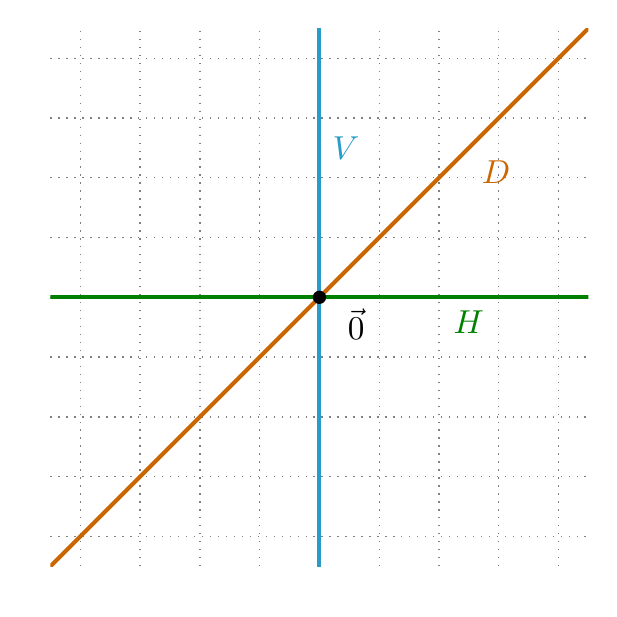
\begin{tikzpicture}[scale=1.2, >=latex]
    \begin{axis}[scale=1,
		    axis equal image,
		    axis line style={draw=none},
		    tick style={draw=none},
		    yticklabels={,,},
		    xticklabels={,,},
		 xmin=-4.5,
		 xmax=4.5,
		 ymin=-4.5,
		 ymax=4.5,
		 major grid style={dotted, gray},
                 xtick={-10,-9,...,10},
                 ytick={-10,-9,...,10},
                 grid=both,
		 anchor=origin]

	    \draw[Green, very thick] (-5,0) -- (5,0) node[near end, below] {$H$};
	    \draw[cyan!80!black, very thick] (0,-5) -- (0,5) node[near end, right] {$V$};
	    \draw[orange!80!black, very thick] (-5,-5) -- (5,5) node[near end, below right] {$D$};


	    \fill[fill=black] (0,0) circle[radius=2pt] node[below right, xshift=5pt] {\color{black}$\vec 0$};
    \end{axis}
\end{tikzpicture}
		\end{solution}
		\item $N=\left\{\vec x\in\R^2:\vec x=t\begin{bmatrix}1\\1\end{bmatrix}\text{ for all }t\in\R\right\}$.
				\begin{solution}[inline]
			$N=\{\}$.
		\end{solution}

		\item $V\cup H$.
			\begin{solution}[inline]
			$V\cup H$ looks like a ``$+$'' going through the origin.
		\end{solution}
		\item $V\cap H$.
			\begin{solution}[inline]
				$V\cap H=\{\vec 0\}$ is just the origin.
		\end{solution}
		\item Does $V\cup H=\R^2$?
			\begin{solution}
				No. $V\cup H$ does not contain $\mat{1\\1}$ while $\R^2$ does contain
				$\mat{1\\1}$.
			\end{solution}
	\end{parts}

\section*{Vector Combinations}
	\vspace{-1em}

	\begin{definition}[Linear Combination]
		A \emph{linear combination} of the vectors $\vec v_1,\vec v_2,\ldots,\vec v_n$ is
		a vector
		\[
			\vec w = \alpha_1\vec v_1+\alpha_2\vec v_2+\cdots+\alpha_n\vec v_n.
		\]
		The scalars $\alpha_1,\alpha_2,\ldots,\alpha_n$ are called the \emph{coefficients} of the linear combination.
	\end{definition}

	\question
	\label{ProbSkewBasis}
	\begin{annotation}
		\begin{goals}
			\Goal{Practice linear combinations.}
			
			The goal of this problem is to
			\begin{itemize}
				\item Practice using the formal term \emph{linear combination}.
				\item Foreshadow span.
			\end{itemize}
		\end{goals}

		\begin{notes}
			\begin{itemize}
				\item In 2, the question should arise: ``Is $3\vec v_1$
					a linear combination of $\vec v_1$ \emph{and}
					$\vec v_2$?'' Address this.
				\item Refer to the magic carpet ride for 5. You don't
					need to do a full proof.
			\end{itemize}
		\end{notes}
	\end{annotation}
	Let $\vec v_1=\begin{bmatrix}1\\1\end{bmatrix}$, $\vec v_2=\begin{bmatrix}1\\-1\end{bmatrix}$, and $\vec w=2\vec v_1+\vec v_2$.
	\begin{parts}
		\item Write $\vec w$ as a column vector. When $\vec w$ is written as a linear combination of $\vec v_1$ and $\vec v_2$, what
			are the coefficients of $\vec v_1$ and $\vec v_2$?
		\begin{solution}
			$\vec w=\mat{3\\2}$; the coefficients are $(2,1)$.
		\end{solution}
		\item Is $\mat{3\\3}$ a linear combination of $\vec v_1$ and $\vec v_2$?
		\begin{solution}[inline]
			Yes. $\mat{3\\3}=3\vec v_1+0\vec v_2$.
		\end{solution}

		\item Is $\mat{0\\0}$ a linear combination of $\vec v_1$ and $\vec v_2$?
		\begin{solution}[inline]
			Yes. $\vec 0=0\vec v_1+0\vec v_2$.
		\end{solution}
		\item Is $\mat{4\\0}$ a linear combination of $\vec v_1$ and $\vec v_2$?
		\begin{solution}[inline]
			Yes. $\mat{4\\0}=2\vec v_1+2\vec v_2$.
		\end{solution}
		\item Can you find a vector in $\R^2$ that isn't a linear combination of
		$\vec v_1$ and $\vec v_2$?
		\begin{solution}
			No. $\mat{1\\0}=\tfrac{1}{2}\vec v_1+\tfrac{1}{2}\vec v_2$ and
			 $\mat{0\\1}=\tfrac{1}{2}\vec v_1-\tfrac{1}{2}\vec v_2$. Therefore
			 \[
				 \mat{a\\b}=a\mat{1\\0}+b\mat{0\\1} = a(\tfrac{1}{2}\vec v_1+\tfrac{1}{2}\vec v_2)
				 +b(\tfrac{1}{2}\vec v_1-\tfrac{1}{2}\vec v_2)
				 =(\tfrac{a+b}{2})\vec v_1+(\tfrac{a-b}{2})\vec v_2.
			\]
			Therefore any vector in $\R^2$ can be written as linear combinations
			of $\vec v_1$ and $\vec v_2$.
		\end{solution}
		\item Can you find a vector in $\R^2$ that isn't a linear combination of
		$\vec v_1$?
		\begin{solution}
			Yes. All linear combinations of $\vec v_1$ have equal $x$ and $y$ coordinates,
			therefore $\vec w=\mat{2\\1}$ is not a linear combination of $\vec v_1$.
		\end{solution}
	\end{parts}


	\question
	\begin{annotation}
		\begin{goals}
			\Goal{Practice formal writing.}
		\end{goals}

		\begin{notes}
			\begin{itemize}
				\item Make everyone \emph{write}. They will think
					they can do it, but they will find it hard if
					they try.
			\end{itemize}
		\end{notes}
	\end{annotation}
	Recall the \emph{Magic Carpet Ride} task where the hover board could travel in the direction
	$\vec h=\mat{3\\1}$ and the magic carpet could move in the direction $\vec m=\mat{1\\2}$.
	\begin{parts}
		\item Rephrase the sentence \emph{``Gauss can be reached using just the magic carpet and the 
			hover board''} using formal mathematical language.
			\begin{solution}
				Gauss's location can be written as a linear combination of $\vec m$ and $\vec h$.
			\end{solution}
		\item Rephrase the sentence \emph{``There is nowhere Gauss can hide where he is inaccessible
			by magic carpet and hover board''} using formal mathematical language.
			\begin{solution}
				Every vector in $\R^2$ can be written as a linear combination of $\vec m$ and
				$\vec h$.
			\end{solution}
		\item Rephrase the sentence \emph{``$\R^2$ is the set of all linear combinations of $\vec h$ and $\vec m$''}
			using formal mathematical language.
			\begin{solution}
				$\R^2=\{\vec v:\vec v=t\vec m+s\vec h\text{ for some }t,s\in \R\}$.
			\end{solution}
	\end{parts}

\begin{lesson}
	\newpage
	\Title{Restricted Linear Combinations, Lines}

	\Heading{Textbook}
	Section 1.2

	\Heading{Objectives}
	\begin{itemize}
		\item Read and digest a new definition.
		\item Use pictures to explore a new concept.
		\item Convert from an equation-representation of a line
			to a set-representation.
	\end{itemize}

	\Heading{Motivation}
	Part of doing math in the world is reading and understanding other people's
	definitions. Most students will not have heard of non-negative linear combinations
	or convex linear combinations. This is a chance for them to read and try to understand
	these formal definitions. They will need to draw pictures to get an intuition 
	about what these concepts mean.

	These concepts are useful in their own right, and in particular, convex linear
	combinations can be used to describe line segments. Adding these definitions to 
	a student's toolbox serves the goal of \emph{being able to describe the world with
	mathematics}.

	To that end, we start working with lines. Lines are something students have
	used since grade school, but they worked with them in $y=mx+b$ form which is
	only applicable in $\R^2$. We want to convert this representation into
	vector form and set-based descriptions which apply to all dimensions.

	\newpage
\end{lesson}
	\begin{definition}[Non-negative \& Convex Linear Combinations]
		The linear combination $\vec w=\alpha_1\vec v_1+\alpha_2\vec v_2+\cdots+\alpha_n\vec v_n$ is
		called a \emph{non-negative} linear combination of $\vec v_1,\vec v_2,\ldots,\vec v_n$ if
		$\alpha_1,\alpha_2,\ldots,\alpha_n\geq 0$. 
		
		If $\alpha_1,\alpha_2,\ldots,\alpha_n\geq 0$
		and $\alpha_1+\alpha_2+\cdots+\alpha_n=1$, then $\vec w$ is called a \emph{convex} linear combination
		of  $\vec v_1,\vec v_2,\ldots,\vec v_n$.
	\end{definition}

	\question
	\begin{annotation}
		\begin{goals}
			\Goal{Geometric meaning of \emph{non-negative} and \emph{convex}
			linear
			combinations.}
			
			The goal of this problem is to
			\begin{itemize}
				\item Read and apply the definition of non-negative and convex
					linear combinations.
				\item Gain geometric intuition for non-negative and convex linear
					combinations.
				\item Learn how to describe line segments using
					convex linear combinations.
			\end{itemize}
		\end{goals}

		\begin{notes}
			\begin{itemize}
				\item This question is about reading and applying;
					emphasize that before they start.
				\item The geometry won't be obvious. Ask them to \emph{draw} specific
					linear combinations (e.g., $(1/2,1/2)$) to get an idea.
				\item They know $\vec a$ and $\vec b$ span all vectors from problem \ref{ProbSkewBasis}.
				\item In part 1, they will forget $\vec a$ and $\vec b$ are linear combinations of themselves.
				\item Part 2 (b) highlights a degeneracy that will come up again when discussing linear independependence
					and dependence. Explain how the picture for non-negative linear combinations
					almost always looks one way, but this case is an exception.
			\end{itemize}
		\end{notes}
	\end{annotation}
	Let
	\[
		\vec a=\mat{1\\1}\qquad \vec b=\mat{-1\\1}\qquad \vec c=\mat{0\\1}\qquad\vec d=\mat{0\\2}\qquad\vec e=\mat{-1\\-1}.
	\]
	\begin{parts}
		\item Out of $\vec a$, $\vec b$, $\vec c$, $\vec d$, and $\vec e$, which
			vectors are
			\begin{enumerate}
				\item linear combinations of $\vec a$ and $\vec b$?
				\begin{solution}[inline]
					All of them, since $\Span\{\vec a,\vec b\}=\R^2$.
				\end{solution}

				\item non-negative linear combinations of $\vec a$ and $\vec b$?
				\begin{solution}[inline]
					$\vec a$, $\vec b$, $\vec c$, $\vec d$.
				\end{solution}

				\item convex linear combinations of $\vec a$ and $\vec b$?
				\begin{solution}[inline]
					$\vec a$, $\vec b$, $\vec c$.
				\end{solution}
			\end{enumerate}

		\item If possible, find two vectors $\vec u$ and $\vec v$ so that
			\begin{enumerate}
				\item $\vec a$ and $\vec c$ are non-negative linear combinations
					of $\vec u$ and $\vec v$ but $\vec b$ is not.
				\begin{solution}
					Let $\vec u=\vec a$ and $\vec v=\vec c$.
				\end{solution}

				\item $\vec a$ and $\vec e$ are non-negative linear combinations
					of $\vec u$ and $\vec v$.
				\begin{solution}
					Let $\vec u=\vec a$ and $\vec v=\vec e$.
				\end{solution}

				\item $\vec a$ and $\vec b$ are non-negative linear combinations
					of $\vec u$ and $\vec v$ but $\vec d$ is not.
				\begin{solution}
					Impossible. If $\vec a$ and $\vec b$ are non-negative
					linear combinations of $\vec u$ and $\vec v$, then every non-negative
					linear combination of $\vec a$ and $\vec b$ is also a non-negative
					linear combination of $\vec u$ and $\vec v$. And, we already concluded that
					$\vec d$ is a non-negative linear combination of $\vec a$ and $\vec b$.
				\end{solution}

				\item $\vec a$, $\vec c$, and $\vec d$ are convex linear
					combinations of $\vec u$ and $\vec v$.
				\begin{solution}
					Impossible. Convex linear combinations all lie on the same line segment,
					but $\vec a$, $\vec c$, and $\vec d$ are not collinear.
				\end{solution}
			\end{enumerate}Otherwise, explain why it's not possible.
	\end{parts}

\section*{Lines and Planes}

	\question
	Let $A$ be the set of points $(x,y)\in\R^2$ such that $y=2x+1$.
	\begin{parts}
		\item Describe $A$ using set-builder notation.
		\item Draw $A$ as a subset of $\R^2$.
		\item Add the vectors $\vec a=\mat{-1\\-1}$, $\vec b=\mat{1\\3}$ and
			$\vec d=\vec b-\vec a$ to your drawing.
		\item For which $t\in\R$ is it true that $\vec a+t\vec d\in A$? Explain using your picture.
	\end{parts}

\begin{lesson}
	\newpage
	\Title{Vector Form of Lines, Intersecting Lines}

	\Heading{Textbook}
	Section 1.2

	\Heading{Objectives}
	\begin{itemize}
		\item Fluency with vector form of a line in $\R^2$ and $\R^3$.
		\item Recognize that vector form of a line is not unique.
		\item Find the intersection of two lines in vector form.
	\end{itemize}

	\Heading{Motivation}
	A single linear equation cannot describe a line in more than two dimensions.
	One way to describe a line that works in all dimensions is vector form, which
	is a shorthand for a particular set. Vector form has the upside that it makes it easy
	to produce points on a line, but it has the downside that it is not unique.

	Vector form works because a line in any dimension can be defined by two
	points or, equivalently, a point and a direction. Though we don't yet have
	a systematic way to write solutions to a system of linear equations,
	if we have a system representing a line, all we need to do is guess two
	solutions to that system to find vector form of the line.


	\begin{annotation}
		\begin{notes}
			The biggest stumbling block for finding the intersection of two lines
			in vector form will be choosing different dummy variables before
			setting the lines equal. 
		\end{notes}
	\end{annotation}
	One thing vector form makes difficult is finding intersections, but intersections
	can be turned into just another algebra problem involving a system of equations.

	\newpage
\end{lesson}

	\newpage
	\begin{definition}[Vector Form of a Line]
		A line $\ell$ is written in \emph{vector form} if it is expressed
		as
		\[
			\vec x=t\vec d+\vec p
		\]
		for some vector $\vec d$ and point $\vec p$. That is, $\ell = \{\vec x: \vec x=
		t\vec d+\vec p\text{ for some } t\in\R \}$. The vector 
		$\vec d$ is called a \emph{direction
		vector} for $\ell$.
	\end{definition}

	\question
	Let $\ell\subseteq \R^2$ be the line with equation $2x+y=3$,
	and let $L\subseteq \R^3$ be the line with equations $2x+y=3$ and
	$z=y$.
	\begin{parts}
		\item Write $\ell$ in vector form. Is vector form of $\ell$ unique?
		\item Write $L$ in vector form. 
		\item Find another vector form for $L$ where both ``$\vec d$'' and
			``$\vec p$'' are different from before.
	\end{parts}

	\question
	Let $A$, $B$, and $C$ be given in vector form by 
	\[\overbrace{\vec x=t\mat{1\\2\\3}+\mat{0\\0\\1}}^{\displaystyle A}
	\qquad \overbrace{\vec x=t\mat{-1\\1\\1}+\mat{-1\\1\\2}}^{\displaystyle B}
	\qquad \overbrace{\vec x=t\mat{2\\-1\\1}+\mat{1\\1\\1}}^{\displaystyle C}.
	\]
	\begin{parts}
		\item Do the lines $A$ and $B$ intersect? Justify your conclusion.
		\item Do the lines $A$ and $C$ intersect? Justify your conclusion.
		\item Let $\vec p\neq \vec q$ and suppose
			$X$ has vector form $\vec x=t\vec d+\vec p$ and $Y$ has
			vector form $\vec x=t\vec d+\vec q$. Is it possible
			that $X$ and $Y$ intersect?
	\end{parts}
	

\begin{lesson}
	\newpage
	\Title{Planes, Span}

	\Heading{Textbook}
	Section 1.2

	\Heading{Objectives}
	\begin{itemize}
		\item Describe a plane in vector form.
		\item Visualize spans.
		\item Recognize the dimension of $\Span(X)$ is not necessarily how many vectors
			are in $X$.
		\item Define \emph{span}.
	\end{itemize}

	\Heading{Motivation}
	Planes are just like lines but one dimension hire. Vector form of a plane is just like
	vector form of a plane with all the advantages and disadvantages. But, we now have
	\emph{two} direction vectors.

	Spans are similar to lines and planes; $\Span\{\vec a,\vec b\}$ looks a lot like
	vector form of the plane
	$\vec x=t\vec a+s\vec b$. Except, $\Span\{\vec a,\vec b\}$ may not always be a plane.
	We haven't defined linear independence and linear dependence yet, but we will continue to
	foreshadow it by seeing that the dimension of the span of a set is not always the size of
	that set.

	Knowing definitions is an essential part of solving math problems. Span is
	the first definition that students will think they ``know'' but won't be
	able to write down.

	\newpage
\end{lesson}

	\begin{definition}[Vector Form of a Plane]
		A plane $\mathcal P$ is written in \emph{vector form} if it is expressed
		as
		\[
			\vec x=t\vec d_1 +s\vec d_2+\vec p
		\]
		for some vectors $\vec d_1$ and $\vec d_2$ and 
		point $\vec p$. That is, $\mathcal P = \{\vec x: \vec x=
		t\vec d_1+s\vec d_2 +\vec p\text{ for some } t,s\in\R \}$. The vectors 
		$\vec d_1$ and $\vec d_2$ are called \emph{direction
		vectors} for $\mathcal P$.
	\end{definition}

	\question
	Recall the lines $A$ and $B$ given in vector form by
	\[\overbrace{\vec x=t\mat{1\\2\\3}+\mat{0\\0\\1}}^{\displaystyle A}
	\qquad \overbrace{\vec x=t\mat{-1\\1\\1}+\mat{-1\\1\\2}}^{\displaystyle B}.
	\]
	Let $\mathcal P$ the plane that contains the lines $A$ and $B$.
	\begin{parts}
		\item Find two direction vectors in $\mathcal P$.
		\item Write $\mathcal P$ in vector form.
		\item Describe how vector form of a plane relates to linear
			combinations.
		\item Write $\mathcal P$ in vector form using different
			direction vectors and a different point.
	\end{parts}

	\question
	Let $\mathcal Q\subseteq \R^3$ be a plane with equation $x+y+z=1$.
	\begin{parts}
		\item Find three points in $\mathcal Q$.
		\item Find two direction vectors for $\mathcal Q$.
		\item Write $\mathcal Q$ in vector form.
	\end{parts}

\section*{Span}
	\begin{definition}[Span]
		The \emph{span} of a set of vectors $V$ is the set of
		all linear combinations of vectors in $V$.  That is,
		\[
			\Span V = \{\vec v:\vec v=\alpha_1\vec v_1+\alpha_2\vec v_2 + \cdots 
			+\alpha_n\vec v_n\text{ for some }\vec v_1,\vec v_2,\ldots,\vec v_n\in V
			\text{ and scalars }\alpha_1,\alpha_2,\ldots,\alpha_n\}.
		\]
	\end{definition}

	\question
	Let $\vec v_1=\mat{1\\1}$, $\vec v_2=\mat{1\\-1}$, and $\vec v_3=\mat{2\\2}$.
	\begin{parts}
		\item Draw $\Span\{\vec v_1\}$.
		\item Draw $\Span\{\vec v_2\}$.
		\item Describe $\Span\{\vec v_1,\vec v_2\}$.
		\item Describe $\Span\{\vec v_1,\vec v_3\}$.
		\item Describe $\Span\{\vec v_1,\vec v_2,\vec v_3\}$.
	\end{parts}


\begin{lesson}
	\newpage
	\Title{Span, Translated Span}

	\Heading{Textbook}
	Section 1.2

	\Heading{Objectives}
	\begin{itemize}
		\item Explain why spans always go through the origin.
		\item Express lines or planes through the origin as spans.
		\item Express lines or planes not through the origin as translated spans.
	\end{itemize}

	\Heading{Motivation}
	Translated spans link vector form of lines and planes with sets and spans.
	Soon we will have the vocabulary of linear independence and be able to
	talk about independent direction vectors of a plane, but right now just connecting
	the concepts and notation is enough.

	\newpage
\end{lesson}

	\question
	Let $\ell_1\subseteq \R^2$ be the line with equation $x-y=0$ and $\ell_2\subseteq\R^2$
	the line with equation $x-y=4$.
	\begin{parts}
		\item If possible, describe $\ell_1$ as a span. Otherwise explain why it's not possible.
		\item If possible, describe $\ell_2$ as a span. Otherwise explain why it's not possible.
		\item Does the expression $\Span(\ell_1)$ make sense? If so, what is it? How about
			$\Span(\ell_2)$?
	\end{parts}


	\begin{definition}[Set Addition]
		If $A$ and $B$ are sets of vectors, then the \emph{set sum} of $A$
		and $B$, denoted $A+B$, is
		\[
			A+B=\{\vec x:\vec x=\vec a+\vec b\text{ for some }\vec a\in A\text{ and }
			\vec b\in B\}.
		\]
	\end{definition}

	\question
	Let $A=\left\{\mat{1\\2}\right\}$, $B=\left\{\mat{1\\1},\mat{1\\-1}\right\}$, 
	and $\ell=\Span\left\{\mat{1\\-1}\right\}$.
	\begin{parts}
		\item Draw $A$, $B$, and $A+B$ in the same picture.
		\item Is $A+B$ the same as $B+A$?
		\item Draw $\ell+A$.
		\item Consider the line $\ell_2$ given in vector form by $\vec x=t\mat{1\\-1}+\mat{1\\2}$.
			Can $\ell_2$ be described using only a span? What about using a span
			and set addition?
	\end{parts}


	
\begin{lesson}
	\newpage
	\Title{Linear Independence \& Dependence}

	\Heading{Textbook}
	Section 1.2

	\Heading{Objectives}
	\begin{itemize}
		\item Define linear independence/dependence using spans.
		\item Pick linearly independent subsets with the same span by inspection.
		\item Explain why having a ``closed loop'' or trivial linear combination
			means a set is linearly dependent.
	\end{itemize}

	\Heading{Motivation}
	Linear independence/dependence is one of the biggest concepts in linear algebra. 
	Linear independence/dependence tells us whether a set has redundant information
	in it with respect to spans. The idea of a having redundant information vs\mbox{.}
	not comes up all the time in the world (sometimes it's a plus, sometimes it's not).
	
	Knowing
	a set is independent tells us what its span will look like (in terms of what dimension
	it will be). It is also an abstract concept that has both a ``geometric'' definition
	and an ``algebraic'' one. 
	\begin{annotation}
		\begin{notes}
			Don't define a linearly dependent \emph{set}, define
			a linearly dependent \emph{list}. Otherwise you cannot talk about
			$\mat{1\\1}$ and $\mat{1\\1}$ be linearly dependent since sets don't
			contain duplicates.
		\end{notes}
	\end{annotation}
	Geometrically, a set is linearly dependent if you can remove
	a vector without the span changing. Algebraically a set is linearly dependent if there
	is a non-trivial linear combination giving the zero vector. This lesson focuses on the
	geometric definition (with the algebraic definition coming next).

	Though the algebraic definition is easier to work with in proofs, the geometric definition
	provides intuition about how to visualize linearly
	dependent sets.

	\newpage
\end{lesson}
\newpage
\pagestyle{iola}
\section*{Task 1.3: The Magic Carpet, Getting Back Home}
\addcontentsline{toc}{subsection}{Task 1.3: The Magic Carpet Ride, Getting Back Home}

Suppose you are now in a three-dimensional world for the carpet
ride problem, and you have three modes of transportation:
\[
	\vec v_1 = \mat{1 \\1 \\ 1}\qquad
	\vec v_2 = \mat{6 \\3 \\ 8}\qquad
	\vec v_3 = \mat{4 \\1 \\ 6}
\]

You are only allowed to use each mode of transportation \textbf{once}
(in the forward or backward direction) for a fixed amount of time ($c_1$
on $\vec v_1$, $c_2$ on $\vec v_2$, $c_3$ on $\vec v_3$).

\vspace{5mm}


\begin{enumerate}
	\item  Find the amounts of time on
each mode of transportation ($c_1$, $c_2$,  and $c_3$, respectively)
needed to go on a journey that starts and ends at home \emph{or} explain why
it is not possible to do so.

	\item Is there more than one way to make a journey that meets the
	requirements described above? (In other words, are there different
	combinations of times you can spend on the modes of transportation so
	that you can get back home?) If so, how?

	\item Is there anywhere in this 3D world that Gauss
	  could hide from you? If so, where? If not, why not?

	\item What is $\Span \left\{\mat{1 \\1 \\  1},\mat{6 \\3 \\ 8},\mat{4  \\1 \\ 6} \right\}$?

\end{enumerate}


\newpage
\pagestyle{siefken}


	\newpage
	\begin{definition}[Linearly Dependent \& Independent]
		We say the vectors $\vec v_1,\vec v_2,\ldots,\vec v_n$ are
		\emph{linearly dependent} if for at least one $i$,
		\[
			\vec v_i\in\span\{\vec v_1,\vec v_2,\ldots,\vec v_{i-1},
			\vec v_{i+1},\ldots,\vec v_n\}.
		\]
		Otherwise, they are called \emph{linearly independent}.
	\end{definition}

	\question
		Let $\vec u=\mat{1\\0\\0}$, $\vec v=\mat{0\\1\\0}$, and $\vec w=\mat{1\\1\\0}$.
	\begin{parts}
		\item Describe $\Span\{\vec u,\vec v,\vec w\}$.
		\item Is $\{\vec u,\vec v,\vec w\}$ linearly independent?  Why or why not?
	\end{parts}

	Let $X=\{\vec u,\vec v,\vec w\}$.

	\begin{parts}[resume]
		\item Give a subset $Y\subseteq X$ so that $\Span Y=\Span X$ and $Y$ is
		linearly independent.
		\item Give a subset $Z\subseteq X$ so that $\Span Z=\Span X$ and $Z$ is
		linearly independent and $Z\neq Y$.
	\end{parts}


	\begin{definition}[Trivial Linear Combination]
	We say a linear combination 
	$a_1\vec v_1+a_2\vec v_2+\cdots +a_n\vec v_n$
	is \emph{trivial} if $a_1=a_2=\cdots=a_n=0$.
	\end{definition}
	
	\question
		Recall $\vec u=\mat{1\\0\\0}$, $\vec v=\mat{0\\1\\0}$, and $\vec w=\mat{1\\1\\0}$.
	\begin{parts}
		\item Consider the linearly dependent 
		set $\{\vec u,\vec v,\vec w\}$ (where $\vec u,\vec v,\vec w$
		are defined as above).  Can you write $\vec 0$
		as a non-trivial linear combination of vectors in this set?
		\item Consider the linearly independent 
		set $\{\vec u,\vec v\}$.  Can you write $\vec 0$
		as a non-trivial linear combination of vectors in this set?
	\end{parts}


\begin{lesson}
	\newpage
	\Title{Linear Independence \& Dependence---Equivalent Definitions}

	\Heading{Textbook}
	Section 1.2

	\Heading{Objectives}
	\begin{itemize}
		\item Define linear independence/dependence in terms of trivial linear combinations.
		\item Explain how the geometric and algebraic definitions of linear independence/dependence relate.
		\item Explain the connection between a vector equation having multiple
			solutions and those vectors being linearly independent/dependent.
		\item Identify the largest linearly independent set that could exist in $\R^n$.
	\end{itemize}

	\Heading{Motivation}
	We've done geometry, now let's do algebra. The geometric and algebraic definitions
	are equivalent, but they suggest different consequences. The geometric definition
	of linear independence tells us about the dimension of a span. The algebraic
	definition tells us about the number of solutions to a vector equation.

	\newpage
\end{lesson}

	We now have an equivalent definition of linear dependence.

	\begin{definition}[Linearly Dependent \& Independent]
	The vectors $\vec v_1,\vec v_2,\ldots,\vec v_n$ are
	\emph{linearly dependent} if there is a non-trivial
	linear combination of $\vec v_1,\ldots,\vec v_n$ that
	equals the zero vector.
	\end{definition}

	\question
	\begin{parts}
		\item Explain how this new definition implies the old one.
		\item Explain how the old definition implies this new one.
	\end{parts}

	Since we have old def $\implies$ new def, and new def $\implies$ old def ($\implies$
	should be read aloud as `implies'), the two definitions
	are \emph{equivalent} (which we write as new def $\iff$ old def).


	\question
	Suppose for some unknown $\vec u, \vec v, \vec w$, and $\vec a$,
	\[
		\vec a = 3\vec u+2\vec v +\vec w\qquad \text{and}\qquad 
		\vec a = 2\vec u+\vec v -\vec w.
	\]
	\begin{parts}
		\item Could the set $\{\vec u,\vec v,\vec w\}$ be linearly
		independent?
	\end{parts}
	Suppose that
	\[
		\vec a = \vec u+6\vec r-\vec s
	\]
	is the \emph{only} way to write $\vec a$ using $\vec u,\vec r,\vec s$.
	\begin{parts}[resume]
		\item Is $\{\vec u,\vec r,\vec s\}$ linearly independent?
		\item Is $\{\vec u,\vec r\}$ linearly independent?
		\item Is $\{\vec u,\vec v,\vec w,\vec r\}$ linearly independent?
	\end{parts}


\newpage
\pagestyle{iola}
\section*{Task 1.4: Linear Independence and Dependence, Creating Examples}
\addcontentsline{toc}{subsection}{Task 1.4: Linear Independence and Dependence, Creating Examples}



\begin{enumerate}
	\item Fill in the following chart keeping track of the strategies you used to generate
examples.

\vspace{2mm}

\begin{center}
\begin{tabular}{|c|c|c|}
	\hline
	&Linearly independent & Linearly dependent \\
	\hline
	A set of 2 vectors in $\R^2$ &&\\
	\hline
	A set of 3 vectors in $\R^2$ &&\\
	\hline
	A set of 2 vectors in $\R^3$ &&\\
	\hline
	A set of 3 vectors in $\R^3$ &&\\
	\hline
	A set of 4 vectors in $\R^3$ &&\\
	\hline
\end{tabular}
\end{center}
	
		\item Write at least two generalizations that can
			be made from these examples and the strategies you
			used to create them.

\end{enumerate}


\newpage
\pagestyle{siefken}


\begin{lesson}
	\newpage
	\Title{Dot Product, Orthogonality}

	\Heading{Textbook}
	Section 1.3

	\Heading{Objectives}
	\begin{itemize}
		\item Compute the dot product of two vectors.
		\item Compute the length of a vector.
		\item Find the distance between two vectors.
		\item Define what it means for vectors to be orthogonal.
		\item Interpret the sign of the dot product geometrically.
		\item Create a unit vector in the direction of another.
	\end{itemize}

	\Heading{Motivation}
	Studying $\R^n$ we're in a natural inner product space with lengths and
	angles. The dot product allows us to get at lengths and angles. It will
	also give an alternative way to compute matrix products (dot product with rows
	instead of linear combination of columns). 

	Most importantly, the dot product tells us how much two vectors point in
	the same direction as well as when they're orthogonal. 

	\newpage
\end{lesson}


\newpage
\section*{Dot Product}
	\begin{definition}[Norm]
		The \emph{norm} of a vector $\vec v=\mat{v_1\\\vdots\\v_n}$ is the
		length/magnitude of $\vec v$. It is written $\|\vec v\|$ and can be computed from
		the Pythagorean formula
		\[
			\|\vec v\|=\sqrt{v_1^2+\cdots +v_n^2}.
		\]
	\end{definition}

	\begin{definition}[Dot Product]
	If $\vec a=\begin{bmatrix}a_1\\ a_2\\ \vdots \\ a_n\end{bmatrix}$ and 
	$\vec b=\begin{bmatrix}b_1\\ b_2\\ \vdots \\ b_n\end{bmatrix}$ are two vectors in $n$-dimensional
		space, then the \emph{dot product} of $\vec a$ an $\vec b$ is
	\[
		\vec a\cdot\vec b = a_1b_1+a_2b_2+\cdots+a_nb_n.
	\]
	Equivalently, the dot product is defined by the geometric formula
	\[
		\vec a\cdot \vec b = \|\vec a\|\|\vec b\|\cos \theta
	\]
	where $\theta$ is the angle between $\vec a$ and $\vec b$.
	\end{definition}
	
	\question
		Let $\vec a=\begin{bmatrix}1\\1\end{bmatrix}$, $\vec b=\begin{bmatrix}3\\2\end{bmatrix}$, and $\vec u=\begin{bmatrix}1\\2\\1\end{bmatrix}$.
	\begin{parts}
		\item 
		\begin{enumerate}	
			\item Draw a picture of $\vec a $ and $\vec b$.
			\item Compute $\vec a\cdot \vec b$.
			\item Find $\|\vec a\|$ and $\|\vec b\|$ and use your knowledge of
			the multiple ways to compute the dot product to find $\theta$,
			the angle between $\vec a$ and $\vec b$. Label $\theta$ on your picture.
		\end{enumerate}
		\item Draw the graph of $\cos$ and identify which angles make $\cos$ negative, zero,
		or positive.

		\item Draw a new picture of $\vec a$ and $\vec b$ and on that picture draw
		\begin{enumerate}	
			\item a vector $\vec c$ where $\vec c\cdot \vec a$ is negative.
			\item a vector $\vec d$ where $\vec d\cdot \vec a=0$ and $\vec d\cdot \vec b < 0$.
			\item a vector $\vec e$ where $\vec e\cdot \vec a=0$ and $\vec e\cdot \vec b>0$.
			\item Could you find a vector $\vec f$ where $\vec f\cdot \vec a=0$ and $\vec f\cdot \vec b=0$?
			Explain why or why not.
		\end{enumerate}

		\item Recall the vector $\vec u$ whose coordinates are given at the beginning of this problem.
		\begin{enumerate}
			\item Write down a vector $\vec v$ so that the angle between $\vec u$ and $\vec v$
			is $\pi/2$. (Hint, how does this relate to the dot product?)
			\item Write down another vector $\vec w$ (in a different direction from $\vec v$)
			so that the angle between $\vec w$ and $\vec u$ is $\pi/2$.
			\item Can you write down other vectors different than both $\vec v$ and $\vec w$ that still
			form an angle of $\pi/2$ with $\vec u$?  How many such vectors are there?
		\end{enumerate}
	\end{parts}

	\newpage
	\begin{theorem}
		For a vector $\vec v\in \R^n$, the formula
		\[
			\|\vec v\| = \sqrt{\vec v\cdot \vec v}
		\]
		always holds.
	\end{theorem}

	\begin{definition}[Distance]
		The \emph{distance} between two vectors $\vec u$ and $\vec v$ is $\|\vec u-\vec v\|$.
	\end{definition}
	\begin{definition}[Unit Vector]
		A vector $\vec v$ is called a \emph{unit vector} if $\|\vec v\|=1$.
	\end{definition}
	
	\question
	Let $\vec u=\mat{1\\2\\1}$ and $\vec v=\mat{1\\1\\3}$.
	\begin{parts}
		\item Find the distance between $\vec u$ and $\vec v$.
		\item Find a unit vector in the direction of $\vec u$.
		\item Does there exists a \emph{unit vector} $\vec x$ that is distance
			$1$ from $\vec u$?
		\item Suppose $\vec y$ is a unit vector and the distance between $\vec y$ and
			$\vec u$ is $2$.  What is the angle between $\vec y$ and $\vec u$?
	\end{parts}


	\begin{definition}[Orthogonal]
		Two vectors $\vec u$ and $\vec v$ are \emph{orthogonal} to each other
		if $\vec u\cdot \vec v=0$.  The word orthogonal is synonymous with the
		word perpendicular.
	\end{definition}
	
	\question
	\begin{parts}
		\item Find two vectors orthogonal to $\vec a=\mat{1\\-3}$.  Can you find two such vectors that
			are not parallel?
		\item Find two vectors orthogonal to $\vec b=\mat{1\\-3\\4}$.  Can you find two 
			such vectors that are not parallel?
		\item Suppose $\vec x$ and $\vec y$ are orthogonal to each other and $\|\vec x\|=5$ and $\|\vec y\|=3$.
			What is the distance between $\vec x$ and $\vec y$?
	\end{parts}

\begin{lesson}
	\newpage
	\Title{Normal Form of Lines and Planes}

	\Heading{Textbook}
	Section 1.2

	\Heading{Objectives}
	\begin{itemize}
		\item Describe lines and planes in normal form.
	\end{itemize}

	\Heading{Motivation}
	Physics often describes surfaces in terms of normal and tangential components.
	Normal form of lines and planes is one way to get at this decomposition. Further, thinking
	about lines and planes in terms of right angles will help when visualizing orthogonal projections.

	\newpage
\end{lesson}
	
	\question
	\begin{parts}
		\item Draw $\vec u=\begin{bmatrix}2\\3\end{bmatrix}$ and \emph{all}
		vectors orthogonal to it. Call this set $A$.
		\item If $\vec x=\begin{bmatrix}x\\y\end{bmatrix}$ and $\vec x$ is 
		orthogonal to $\vec u$, what is $\vec x\cdot \vec u$?
		\item Expand the dot product $\vec u\cdot \vec x$ to get an equation
		for $A$.
		\item If possible, express $A$ as a span.
	\end{parts}

	\begin{definition}[Normal Vector]
		A \emph{normal vector} to a line (or plane or hyperplane) is a non-zero vector that is orthogonal to it.
	\end{definition}

	\question
	Let $\vec d=\mat{1\\2}$ and $\vec p=\mat{1\\-1}$, and define the lines
	\[
		\ell_1 = \Span\{\vec d\}\qquad\text{and}\qquad \ell_2=\{\vec p\}+\Span\{\vec d\}.
	\]
	\begin{parts}
		\item Find a vector $\vec n$ that is a normal vector for both $\ell_1$ and
			$\ell_2$.
		\item Let $\vec v\in \ell_1$ and $\vec u\in \ell_2$.
			What is $\vec n\cdot \vec v$? What about $\vec n\cdot \vec u$?
		\item A line is expressed in \emph{normal form} if it is represented by an
			equation of the form $\vec n\cdot (\vec x-\vec q)=0$ for some $\vec n$ and 
			$\vec q$. Express $\ell_1$ and $\ell_2$ in normal form.
	\end{parts}
	
	\question
	Let $\vec n=\mat{1\\1\\1}$.
	\begin{parts}
		\item Use set-builder notation to write down the set, $X$, of
			all vectors orthogonal to $\vec n$. Describe this set
			geometrically.
		\item Describe $X$ using an equation.
		\item Describe $X$ as a span.
	\end{parts}


\begin{lesson}
	\newpage
	\Title{Projections}

	\Heading{Textbook}
	Section 1.4

	\Heading{Objectives}
	\begin{itemize}
		\item Project a vector onto lines and finite sets.
		\item Find the components of one vector in terms of another.
	\end{itemize}

	\Heading{Motivation}
	Projection of a vector onto a set, defined as the closet point in the
	set to the vector, is a general operation used outside of linear algebra.
	However, in the land of linear algebra, we have exact formulas for the
	projection. Projections are a chance to explore a seemingly simple definition
	and see it relate to sets, lines, normal form, and vector form.

	\begin{annotation}
		\begin{notes}
			In this class, we don't write $\Proj_{\vec v}\vec u$,
			i.e., the projection of one vector onto another. We
			instead call this $\Comp_{\vec v}\vec u$. We do this so
			as not to confuse $\Proj_{\{\vec v\}}\vec u$ and
			$\Comp_{\vec v}\vec u$. One is projection onto a singleton.
			The other is $\frac{\vec u\cdot \vec v}{\vec v\cdot \vec v}\vec v$.
		\end{notes}
	\end{annotation}
	$\Comp_{\vec v}\vec u$ is the component of a vector in the direction of another, 
	which is sometimes called the projection of $\vec u$ onto $\vec v$. It relates
	to how much one vector points in the direction of another and
	provides a decomposition of vectors in terms of orthogonal components. 
	

	\newpage
\end{lesson}
\section*{Projections}
	
	\begin{definition}[Projection]
		Let $X$ be a set. The \emph{projection} of the vector $\vec v$
		onto $X$, written $\Proj_X\vec v$, is the closest point to $\vec v$ in $X$.
	\end{definition}

	\question
	Let $\vec a=\mat{1\\0}$, $\vec b=\mat{3\\0}$, $\vec v=\mat{1\\1}$ and
	$\ell=\Span\{\vec a\}$.
	\begin{parts}
		\item Draw $\vec a$, $\vec b$, and $\vec v$ in the same picture.
		\item Find $\Proj_{\{\vec b\}}\vec v$, $\Proj_{\{\vec a,\vec b\}}\vec v$.
		\item Find $\Proj_\ell \vec v$. (Recall that a quadratic $at^2+bt+c$ has a
			minimum at $t=-\tfrac{b}{2a}$).
		\item Is $\vec v-\Proj_\ell \vec v$ a normal vector for $\ell$?
			Why or why not?
	\end{parts}

	\question
	Let $K$ be the line given in vector form by $\vec x=t\mat{1\\2}+\mat{1\\0}$ and let
	$\vec c=\mat{1\\3}$.
	\begin{parts}
		\item Make a sketch with $\vec c$, $K$, and $\Proj_K\vec c$ (you don't need to compute 
		$\Proj_K\vec c$ exactly).
		\item What should $(\vec c-\Proj_K\vec c)\cdot \mat{1\\2}$ be? Explain.
		\item Use your formula from the previous part to find $\Proj_K\vec c$
			\emph{without} computing any distances.
	\end{parts}

	\begin{definition}[Component]
		Let $\vec u$ and $\vec v\neq \vec 0$ be vectors. The 
		\emph{component of $\vec u$ in the $\vec v$ direction}, written $\Comp_{\vec v}\vec u$,
		is the vector in the direction of $\vec v$ so that $\vec u-\Comp_{\vec v}\vec u$
		is orthogonal to $\vec v$.
	\begin{center}
	\usetikzlibrary{patterns,decorations.pathreplacing}
	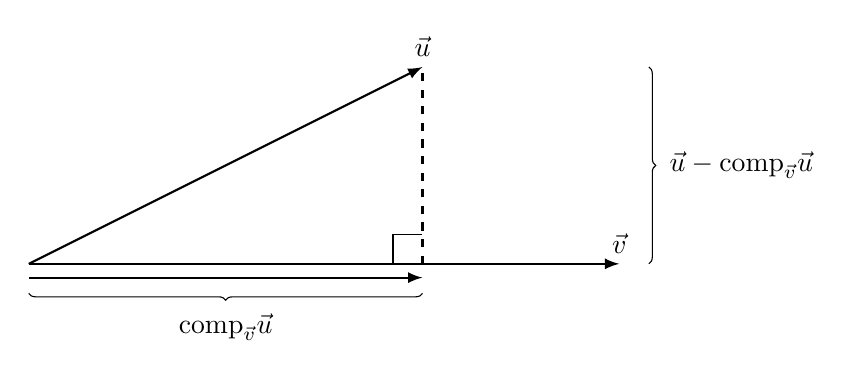
\begin{tikzpicture}[>=latex,scale=2.5]
		\draw[->,thick,black] (0,0) -- (2,1) node [above] {$\vec u$};
		\draw[->,thick,black] (0,0) -- (3,0) node [above] {$\vec v$};
		\draw[->,thick,black,yshift=-.07cm] (0,0) -- (2,0);
		\draw[decoration={brace, mirror}, decorate, yshift=-.15cm] (0,0) -- (2,0) node [midway,below,yshift=-4pt] {$\Comp_{\vec v}\vec u$};
		
		\draw[dashed,thick,black] (2,0) -- (2,1);
		\draw[decoration={brace, mirror}, decorate, xshift=1.15cm] (2,0) -- (2,1) node [midway,right,xshift=4pt] {$\vec u-\Comp_{\vec v}\vec u$};
		\draw[thin,black] (1.85,0)--(1.85,.15)--(2,.15);

	\end{tikzpicture}
	\end{center}
	\end{definition}
	
	\question
	Let $\vec a,\vec b\in \R^3$ be unknown vectors.
	\begin{parts}
		\item List two conditions that $\Comp_{\vec b} \vec a$ must satisfy.
		\item Find a formula for $\Comp_{\vec b}\vec a$.
	\end{parts}


\begin{lesson}
	\newpage
	\Title{Projections, Subspaces}

	\Heading{Textbook}
	Sections 1.2, 1.4

	\Heading{Objectives}
	\begin{itemize}
		\item Identify $\Proj_{\Span\{\vec v\}}\vec u$ with $\Comp_{\vec v}\vec u$.
		\item Identify $\Comp_{\vec v}\vec u$ and $\Comp_{\alpha\vec v}\vec u$
			for all $\alpha\neq 0$, including negative $\alpha$.
		\item Define subspace.
		\item Distinguish subspaces and non-subspaces of $\R^2$.
	\end{itemize}

	\Heading{Motivation}
	Spans are a constructive way to describe lines, planes, and other
	flat objects. Subspaces are a categorical way of defining flat objects.
	Instead of explaining how to find the vectors in a set, we list their
	properties. This is a really powerful idea that facilitates abstraction.

	\begin{annotation}
		\begin{notes}
			\begin{itemize}
			\item	Philosophically, a subspace should be defined
			as a non-empty set closed under linear combinations.
			However, defining it as closed under addition and scalar 
			multiplication gives students new to proofs
			something explicit to hang on to when attempting a proof.
			\item Some people define a subspace as a set containing
			$\vec 0$ and satisfying closure. We define a subspace
			as a non-empty set satisfying closure. We won't be trying
			to trick students by asking if an empty set is a subspace,
			so don't belabor the point.
			\end{itemize}
		\end{notes}
	\end{annotation}
	Since we do not do abstract vector spaces in this course, subspaces are
	the first place (unless you count projections) students will encounter 
	a set defined by its properties. Subspaces are suitable for a first-encounter
	because 1) the properties are simple and familiar and 2) subspaces of $\R^n$
	have a concrete geometric interpretation.

	\newpage
\end{lesson}

	\newpage
	\question
	Let $\vec d=\mat{3\\3}$ and $\vec u=\mat{1\\2}$.
	\begin{parts}
		\item Draw $\vec d$, $\vec u$, $\Span\{\vec d\}$, and $\Proj_{\Span\{\vec d\}}\vec u$
			in the same picture.
		\item How do $\Proj_{\Span\{\vec d\}}\vec u$ and $\Comp_{\vec d}\vec u$ relate?
		\item Compute $\Proj_{\Span\{\vec d\}}\vec u$ and $\Comp_{\vec d}\vec u$.
		\item Compute $\Comp_{-\vec d}\vec u$. Is this the same as or different from 
			$\Comp_{\vec d}\vec u$? Explain.
	\end{parts}


\section*{Subspaces and Bases}
	\vspace{-1em}
	\begin{definition}[Subspace]
		A \emph{subspace} $V\subseteq \R^n$ is a non-empty subset such that
		\begin{enumerate}
			\item[(i)] $\vec u,\vec v\in V$ implies $\vec u+\vec v\in V$.
			\item[(ii)] $\vec u\in V$ implies $k\vec u\in V$ for all scalars $k$.
		\end{enumerate}
	\end{definition}

	Subspaces give a mathematically precise definition of a ``flat space through the origin.''

	\question
	For each set, draw it and explain whether or not it is a subspace of $\R^2$.
	\begin{parts}
		\item $A=\{\vec x\in\R^2:\vec x=\mat{a\\0}\text{ for some }a\in\Z\}$.
		\item $B=\{\vec x\in\R^2:\vec x\neq \mat{0\\0}\}$.
		\item $C=\{\vec x\in\R^2:\vec x=\mat{0\\t}\text{ for some }t\in\R\}$.
		\item $D=\{\vec x\in\R^2:\vec x=\mat{0\\t}+\mat{1\\1}\text{ for some }t\in\R\}$.
		\item $E=\{\vec x\in\R^2:\vec x=\mat{0\\t}\text{ or }\vec x=\mat{t\\0}\text{ for some }t\in\R\}$.
		\item $F=\{\vec x\in\R^2:\vec x=t\mat{3\\1}\text{ for some }t\in\R\}$.
		\item $G=\span\left\{\mat{1\\1}\right\}$.
		\item $H=\span\{\vec u,\vec v\}$ for some unknown vectors $\vec u,\vec v\in\R^2$.
	\end{parts}

\begin{lesson}
	\newpage
	\Title{Basis, Dimension}

	\Heading{Textbook}
	Sections 1.2, 4.3

	\Heading{Objectives}
	\begin{itemize}
		\item Define Basis.
		\item Define Dimension.
		\item Find a basis for a subspace.
		\item Find the dimension of a subspace.
		\item Explain why every vector has a unique representation as a linear
			combination of basis vectors.
	\end{itemize}

	\Heading{Motivation}
	Bases are sets of just enough vectors to describe every vector in a subspace.
	An additional consequence of a basis is that every vector can be \emph{uniquely}
	represented as a linear combination of basis vectors. Using this fact we
	will be able to consider objects in multiple different coordinate systems. However,
	now is the time to get familiar with what a basis is and how to find one.

	Dimension ties the abstract notion of subspace to our intuition about
	Euclidean space. We already know a plane in $\R^3$ is two dimensional,
	but now we know where that number \emph{two} comes from.

	\newpage
\end{lesson}
	\begin{definition}[Basis]
		A \emph{basis} for a subspace $V$ is a linearly independent set of vectors, $\mathcal B$,
		so that $\Span\mathcal B=V$.
	\end{definition}
	\begin{definition}[Dimension]
		The \emph{dimension} of a subspace $V$ is the number of elements in a basis for $V$.
	\end{definition}


	\question
	\begin{annotation}
		\begin{goals}
			\Goal{Apply the definitions of basis and dimension to an easy example.}

			The goal of this problem is to learn
			\begin{itemize}
				\item To apply the definition of basis and dimension.
				\item Intuition that a plane is two dimensional.
				\item A basis is not unique, but always has the same size (this is not proved).
				\item Spans are never bases---you must not confuse a subspace with its basis!
			\end{itemize}
		\end{goals}

		\begin{notes}
			\begin{itemize}
				\item Students will claim $V$ is $\R^2$ and fail to distinguish $\R^2$ and the
					$xy$-plane in $\R^3$.
				\item Parts 2, 3, 4, 6 will be easy; don't belabor them.
				\item Students will fail to distinguish $\Span\{\vec u,\vec v\}$ from $\{\vec u,\vec v\}$. Make sure this distinction
					comes out.
			\end{itemize}
		\end{notes}
	\end{annotation}
	Let $\vec u=\mat{1\\0\\0}$, $\vec v=\mat{0\\1\\0}$, $\vec w=\mat{1\\1\\0}$, and $V=\span\{\vec u,\vec v,\vec w\}$.
	\begin{parts}
		\item Describe $V$.
			\begin{solution}
				$V$ is the $xy$-plane in $\R^3$.
			\end{solution}
		\item Is $\{\vec u,\vec v,\vec w\}$ a basis for $V$?  Why or why not?
			\begin{solution}
				No. The set $\{\vec u,\vec v,\vec w\}$ is linearly dependent since $\vec w=\vec u+\vec v$.
			\end{solution}
		\item Give a basis for $V$.
			\begin{solution}
				$\{\vec u,\vec v\}$
			\end{solution}
		\item Give another basis for $V$.
			\begin{solution}
				$\{\vec u,\vec w\}$ or $\{\vec v,\vec w\}$.
			\end{solution}
		\item Is $\Span\{\vec u,\vec v\}$ a basis for $V$?  Why or why not?
			\begin{solution}
				No. $\Span\{\vec u,\vec v\}$ is an infinite set of vectors
				which includes $\vec 0$, so it cannot be linearly independent and
				therefore isn't a basis.
			\end{solution}
		\item What is the dimension of $V$?
			\begin{solution}
				A basis for $V$ has two vectors so it is two dimensional. We also
				know this because $V$ is the $xy$-plane in $\R^3$ and all planes are two
				dimensional.
			\end{solution}
	\end{parts}


	\question
	Let $\vec a=\mat{1\\2\\3}$, $\vec b=\mat{4\\5\\6}$, $\vec c=\mat{7\\8\\8}$ (notice these vectors
	are linearly independent) and 
	let $P=\span\{\vec a,\vec b\}$ and $Q=\span\{\vec b,\vec c\}$.
	\begin{parts}
		\item Give a basis for and the dimension of $P$.
		\item Give a basis for and the dimension of $Q$.
		\item Is $P\cap Q$ a subspace? If so, give a basis for it and its dimension.
		\item Is $P\cup Q$ a subspace? If so, give a basis for it and its dimension.
	\end{parts}


\begin{lesson}
	\newpage
	\Title{Matrices}

	\Heading{Textbook}
	Section 3.1

	\Heading{Objectives}
	\begin{itemize}
		\item Write a system of linear equations as a matrix equation.
		\item Write a matrix equation as a system of linear equations.
		\item Pose familiar problems (e.g., ``find a normal vector'', or 
			``do these planes intersect\mbox{?}'') as matrix-equation
			questions.
	\end{itemize}

	\Heading{Motivation}
	Matrices will soon become a powerful tool to study linear transformations.
	However, we will start out viewing them as a notation to represent
	systems of linear equations. The fact that matrix-vector multiplication
	has two interpretations, as a linear combination of columns or as a dot product
	with rows, already connects geometry and angles with questions about linear combinations.

	\newpage
\end{lesson}
\section*{Matrices}
	
	\question
	Let $A=\mat{1&2\\3&3}$, $\vec x=\mat{x\\y}$, and $\vec b=\mat{-2\\-1}$.
	\begin{parts}
		\item Compute the product $A\vec x$.
		\item Write down a system of equations that corresponds to the matrix equation
			$A\vec x=\vec b$.
		\item Let $\mat{x_0\\y_0}$ be a solution to $A\vec x=\vec b$. Explain what
			$x_0$ and $y_0$ mean in terms of \emph{linear combinations} (hint: think
			about the columns of $A$).
		\item Let $\mat{x_0\\y_0}$ be a solution to $A\vec x=\vec b$. Explain what
			$x_0$ and $y_0$ mean in terms of \emph{intersecting lines} (hint: think
			about systems of equations).
	\end{parts}

	\question
	Let $\vec u=\mat{1\\2\\3}$, $\vec v=\mat{4\\5\\6}$, $\vec w=\mat{7\\8\\9}$.
	\begin{parts}
		\item How could you determine if $\{\vec u,\vec v,\vec w\}$ was a linearly
			independent set?
		\item Can your method be rephrased in terms of a matrix equation? Explain.
	\end{parts}


	\question
	Consider the system represented by
	\[
		\mat{1&-3&0\\0&0&1\\0&0&0}\mat{x\\y\\z}=\vec b.
	\]
	\begin{parts}
		\item If $\vec b=\mat{1\\2\\3}$, is the set of solutions to this system a 
		point, line, plane, or other?
		\item If $\vec b=\mat{1\\1\\0}$, is the set of solutions to this system a 
		point, line, plane, or other?
	\end{parts}

	\question
	Let $\vec d_1=\mat{1\\1\\2}$ and
	$\vec d_2=\mat{-1\\1\\0}$. 
	Let $\mathcal P$ be the plane given in vector form by $\vec x=t\vec d_1+s\vec d_2$.
	Further, suppose $M$ is a matrix so that $M\vec r\in\mathcal P$ for any $\vec r$.
	\begin{parts}
		\item How many rows does $M$ have?
		\item Find such an $M$.
		\item Find necessary and sufficient conditions (phrased as equations) for $\vec n$
			to be a normal vector for $\vec p$.
		\item Find a matrix $K$ so that solutions
			to $K\vec x=\vec 0$ are normal vectors for $\mathcal P$.
			How do $K$ and $M$ relate?
	\end{parts}


\begin{lesson}
	\newpage
	\Title{Change of Basis I}

	\Heading{Textbook}
	Section 4.4

	\Heading{Objectives}
	\begin{itemize}
		\item Write a vector in multiple bases.
		\item Explain what the notation $[\vec v]_{\mathcal B}$ means.
		\item Explain what the notation $\mat{a\\b\\c}_{\mathcal B}$ means.
	\end{itemize}

	\Heading{Motivation}
	One of the most useful ideas in linear algebra is that you can
	represent a vector, a geometric object, with a list of numbers. This
	is done by picking a basis. So far we've implicitly used the standard basis,
	but now we're going to use other bases.

	\begin{annotation}
		\begin{notes}
			So far, we have written $\mat{1\\1}$ to mean
			$\mat{1\\1}_{\mathcal E}$ where $\mathcal E$ is the
			standard basis. We will continue to do this as convenient,
			but if multiple bases are ever involved, we will be careful
			to specify the basis.
		\end{notes}
	\end{annotation}
	Now lists of numbers can mean many different things and can be identified
	with vectors in many ways, so we need some notation to keep things straight.
	It's important now to distinguish when something is a list of numbers (a matrix)
	and when it is a vector. This distinction will arise again when
	we talk about linear transformations and their matrix representations.

	\newpage
\end{lesson}
\section*{Change of Basis \& Coordinates}

	\question
	The fictional town of Oronto is not aligned with the usual
	compass directions. The streets are laid out as follows:
	
\begin{center}
	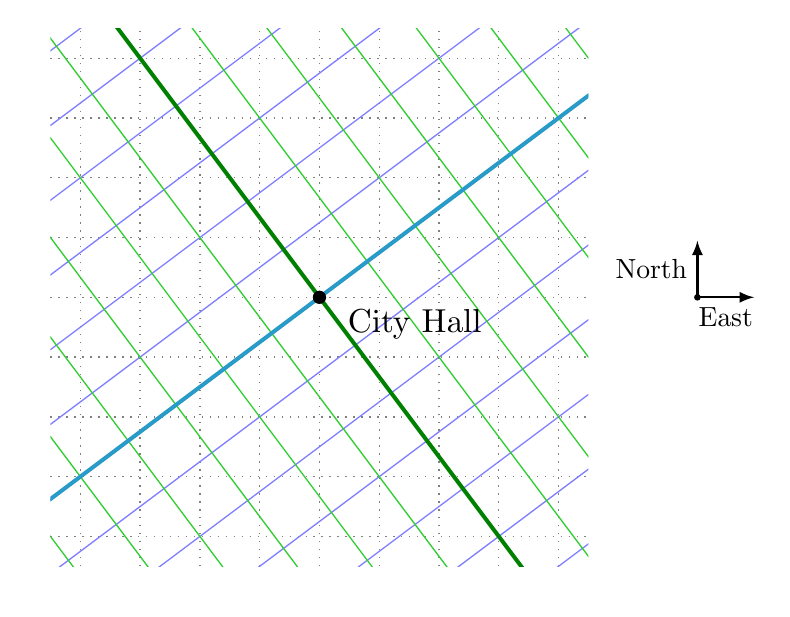
\begin{tikzpicture}[scale=1.2, >=latex]
    \begin{axis}[scale=1,
		    axis equal image,
		    axis line style={draw=none},
		    tick style={draw=none},
		    yticklabels={,,},
		    xticklabels={,,},
		 xmin=-4.5,
		 xmax=4.5,
		 ymin=-4.5,
		 ymax=4.5,
		 major grid style={dotted, gray},
                 xtick={-10,-9,...,10},
                 ytick={-10,-9,...,10},
                 grid=both,
		 anchor=origin]

	    \foreach \ival in {-6,...,6} {
	    	\edef\temp{\noexpand\draw[blue!50!white] (-8-0.6*\ival,-6+0.8*\ival) -- (8-0.6*\ival,6+.8*\ival);}
		\temp
	    }
	    \foreach \ival in {-6,...,6} {
	    	\edef\temp{\noexpand\draw[LimeGreen] (-6+0.8*\ival,8+0.6*\ival) -- (6+0.8*\ival,-8+0.6*\ival);}
		\temp
	    }
	    \draw[Green, very thick] (-6,8) -- (6,-8);
	    \draw[cyan!80!black, very thick] (-8,-6) -- (8,6);


	  \fill[fill=black] (0,0) circle[radius=2pt] node[below right, xshift=5pt] {City Hall};
    \end{axis}
		\draw[->, thick] (4,0) -- (4,.6) node[midway, left] {North};
		\draw[->, thick] (4,0) -- (4.6,0) node[midway, below] {East};
	  \fill[fill=black] (4,0) circle[radius=1pt];
\end{tikzpicture}
\end{center}


	Instead, every street is parallel to
	the vector $\vec d_1=\frac{1}{5}\mat{4\text{ east}\\3\text{ north}}$ or 
	$\vec d_2=\tfrac{1}{5}\mat{-3\text{ east}\\4\text{ north}}$. The center of town
	is City Hall at $\vec 0=\mat{0\text{ east}\\0\text{ north}}$. 

	Locations in Oronto are typically specified in \emph{street coordinates}. That
	is, as a pair $(a,b)$ where $a$ is how far you walk along streets in the $\vec d_1$ direction
	and $b$ is how far you walk in the $\vec d_2$ direction, provided you start at city hall.

	\begin{parts}
		\item The points $A=(2,1)$ and $B=(3,-1)$ are given in street coordinates. Find their  
			east-north coordinates.
		\item The points $X=(4,3)$ and $Y=(1,7)$ are given in east-north coordinates. Find their
			street coordinates.
		\item Define $\vec e_1=\mat{1\text{ east}\\0\text{ north}}$ and 
			$\vec e_2=\mat{0\text{ east}\\1\text{ north}}$. Does $\Span\{\vec e_1,\vec e_2\}
			=\Span\{\vec d_1,\vec d_2\}$?
		\item Notice that $Y=5\vec e_1+5\vec e_2 = \vec d_1+7\vec d_2$. Is the point $Y$
			better represented by the pair $(5,5)$ or by the pair $(1,7)$? Explain.
	\end{parts}

	\begin{definition}[Representation in a Basis]
		Let $\mathcal B=\{\vec b_1,\ldots,\vec b_n\}$ be a basis for a subspace $V$
		and let $\vec v\in V$. The \emph{representation of $\vec v$ in the $\mathcal B$
		basis}, notate $[\vec v]_{\mathcal B}$,
		is the column matrix
		\[
			[\vec v]_{\mathcal B} = \mat{\alpha_1\\\vdots\\\alpha_n}.
		\]
		such that $
			\vec v=\alpha_1\vec b_1+\cdots+\alpha_n\vec b_n.
		$

		Similarly,
		\[
			\mat{\alpha_1\\\vdots\\\alpha_n}_{\mathcal B} = \alpha_1\vec b_1+\cdots +\alpha_n\vec b_n
		\]
		is notation for the linear combination of $\vec b_1,\ldots,\vec b_n$ with coefficients $\alpha_1,\ldots,\alpha_n$.
	\end{definition}

	\question
	Let $\mathcal E=\{\vec e_1,\vec e_2\}$ be the standard basis for $\R^2$ and let 
	$\mathcal C=\{\vec c_1,\vec c_2\}$ where $\vec c_1=\mat{2\\1}_{\mathcal E}$ and $\vec c_2=\mat{5\\3}_{\mathcal E}$
	be another basis for $\R^2$.
	\begin{parts}
		\item Express $\vec c_1$ and $\vec c_2$ as a linear combination of $\vec e_1$ and $\vec e_2$.
		\item Express $\vec e_1$ and $\vec e_2$ as a linear combination of $\vec c_1$ and $\vec c_2$.
		\item Let $\vec v=2\vec e_1+2\vec e_2$. Find $[\vec v]_{\mathcal E}$ and $[\vec v]_{\mathcal C}$.
		\item Can you find a matrix $X$ so that $X[\vec w]_{\mathcal C} = [\vec w]_{\mathcal E}$ for any
			$\vec w$?
		\item Can you find a matrix $Y$ so that $Y[\vec w]_{\mathcal E} = [\vec w]_{\mathcal C}$ for any
			$\vec w$?
		\item What is $YX$?
	\end{parts}

\begin{lesson}
	\newpage
	\Title{Orientation, Matrix Transformations}

	\Heading{Textbook}
	Section 3.2

	\Heading{Objectives}
	\begin{itemize}
		\item Identify the orientation of ordered bases in $\R^2$.
		\item Given a set of input and output vectors for a 
			linear transformation $L:\R^2\to\R^2$, find 
			a matrix for the transformation.
		\item Given a picture $X$ and its image under a linear transformation,
			find a matrix for the transformation.
	\end{itemize}

	\Heading{Motivation}
	Orientation is a topic that comes up in physics and explains the sign
	of the determinant. We define orientation with an existential statement
	about whether or not certain homeomorphisms exist. The goal is not to
	prove anything rigorously about orientation, but to get students to
	make pictures for themselves of vectors moving.

	The Idea is simple: $n-1$ vectors span a space that partitions $\R^n$ in
	two. Add a vector in the top partition (appropriately ordered) and you get
	a positive orientation; add to the bottom and you get a negative orientation.
	There's no way to get from one to the other without passing through the
	hyperplane. We focus on $\R^2$ so that the pictures are easy to draw. Eventually
	we will compute orientation from the determinant, but it's nice to have
	a grounding in where it comes from.

	While we're thinking dynamically, we can start thinking about transformation.
	We already know how to multiply a matrix and a vector and interpret it in
	two different ways. Now we will add a third: multiplication by a given
	matrix is a transformation from vectors to vectors.

	Most of our study of matrix transformations will be of transformations from $\R^n$
	to $\R^n$, even though non-square matrices can describe other transformations.
	For now we stick with pictures of $\R^2$ since they are easy to draw. Then
	we will generalize to linear transformations.

	\newpage
\end{lesson}

	\begin{definition}[Orientation of a Basis]
		The ordered basis $\mathcal B=\{\vec b_1,\ldots,\vec b_n\}$ is \emph{right-handed}
		or \emph{positively oriented} if it can be continuously transformed 
		to the standard basis (with
		$\vec b_i\mapsto \vec e_i$) while remaining linearly independent
		throughout the transformation. Otherwise, $\mathcal B$ is called
		\emph{left-handed} or \emph{negatively oriented}.
	\end{definition}

	\question
	Let $\{\vec e_1,\vec e_2\}$ be the standard basis for $\R^2$ and let
	$\vec u_{\theta}$ be a unit vector. Let $\theta$ be the angle between $\vec u_{\theta}$ and
	$\vec e_1$ measured counter clockwise.
	\begin{parts}
		\item For which $\theta$ is $\{\vec e_1,\vec u_{\theta}\}$ a linearly independent set?
		\item For which $\theta$ can $\{\vec e_1,\vec u_{\theta}\}$ be continuously
			transformed into $\{\vec e_1,\vec e_2\}$ and remain linearly independent the
			whole time?
		\item For which $\theta$ is $\{\vec e_1,\vec u_{\theta}\}$ right-handed? Left-handed?
		\item For which $\theta$ is $\{\vec u_{\theta},\vec e_1\}$ (in that order) right-handed? 
			Left-handed?
	\end{parts}


\newpage
\pagestyle{iola}
\section*{Task 2.1: Italicizing N}
\addcontentsline{toc}{subsection}{Task 2.1: Italicizing N}

\hfill\begin{tikzpicture}[scale=1.5]
    \begin{axis}[
		    axis equal image,
		    axis line style={draw=none},
		    tick style={draw=none},
		    yticklabels={,,},
		    xticklabels={,,},
		 xmin=-.5,
		 xmax=3.5,
		 ymin=-.5,
		 ymax=5.5,
		 major grid style={dotted, gray, thick},
                 xtick={0,1,2,3},
		 ytick={0,1,2,3,4,5},
                 grid=both]

	 \draw[black, thick] (0,0) -- (0,3) -- (2,0) -- (2,3);
    \end{axis}
\end{tikzpicture}\hfill
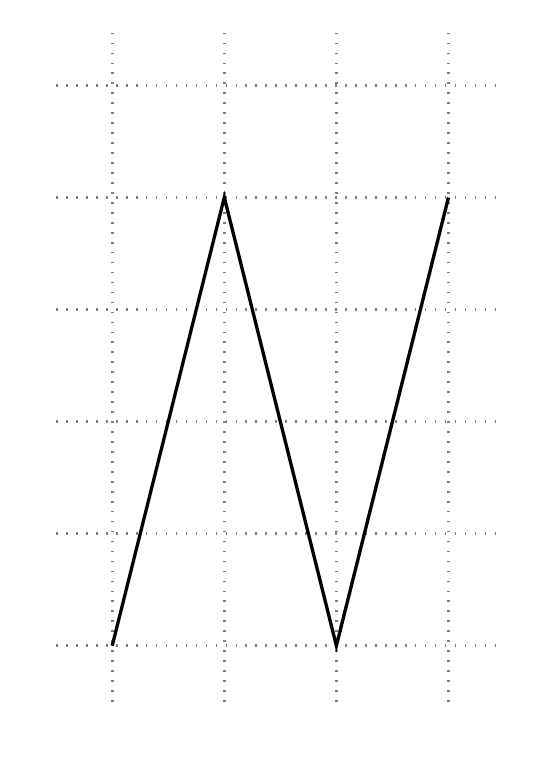
\begin{tikzpicture}[scale=1.5]
    \begin{axis}[
		    axis equal image,
		    axis line style={draw=none},
		    tick style={draw=none},
		    yticklabels={,,},
		    xticklabels={,,},
		 xmin=-.5,
		 xmax=3.5,
		 ymin=-.5,
		 ymax=5.5,
		 major grid style={dotted, gray, thick},
                 xtick={0,1,2,3},
		 ytick={0,1,2,3,4,5},
                 grid=both]

	 \draw[black, thick] (0,0) -- (1,4) -- (2,0) -- (3,4);
    \end{axis}
\end{tikzpicture}\hfill

Suppose that the ``N'' on the left is written in regular 12-point font.  Find a matrix $A$ that will transform
	the ``N'' into the letter on the right which is written in an \emph{italic} 16-point font.

Work with your group to write out your solution and approach.  Make a list of any assumptions you
notice your group making or any questions for further pursuit.
\newpage


\begin{lesson}
	\newpage
	\Title{Linear Transformations I}

	\Heading{Textbook}
	Section 1.2

	\Heading{Objectives}
	\begin{itemize}
		\item 
	\end{itemize}

	\Heading{Motivation}

	\newpage
\end{lesson}
\section*{Task 2.2: Beyond the N}
\addcontentsline{toc}{subsection}{Task 2.2: Beyond the N}

	A few students were wondering how letters placed in other
locations in the plane would be transformed under $A= \mat{ 1&  1/3  \\ 0 & 4/3}$. 
	If an ``E'' is placed around the
	``N,'' the students argued over four different possible results for the
	transformed E's. Which choice below, if any, is correct, and why? If none of
	the four options are correct, what would the correct option be, and why?



\begin{minipage}{6.5in}
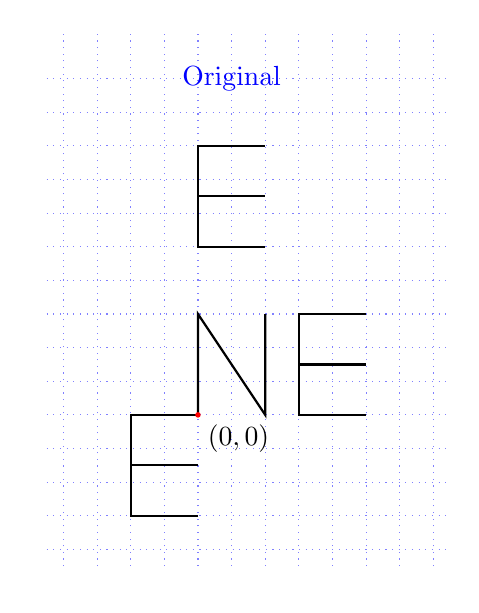
\begin{tikzpicture}
    \begin{axis}[scale=1.2,
		    axis equal image,
		    axis line style={draw=none},
		    tick style={draw=none},
		    yticklabels={,,},
		    xticklabels={,,},
		 xmin=-4.5,
		 xmax=7.5,
		 ymin=-4.5,
		 ymax=11.5,
		 major grid style={dotted, blue!50!white},
                 xtick={-10,-9,...,10},
                 ytick={-10,-9,...,10},
                 grid=both]
	 \draw[black, thick] (0,0) -- (0,3) -- (2,0) -- (2,3);

	 \draw[black, thick] (0,0) -- (-2,0) -- (-2,-3) -- (0,-3)(-2,-1.5) -- (0,-1.5);

	\draw[black, thick] (5, 3) -- (3, 3) -- (3, 0) -- (5, 0)  (3, 1.5) -- (5, 1.5);
	    \draw[black, thick] (2, 8) -- (0, 8) -- (0, 5) -- (2, 5)  (0, 6.5) -- (2, 6.5);

	    \node[blue] at (1,10) {Original};
	    \fill[red] (0,0) circle[radius=1pt] node[below right, black] {$(0,0)$};

    \end{axis}
\end{tikzpicture}
\hfill
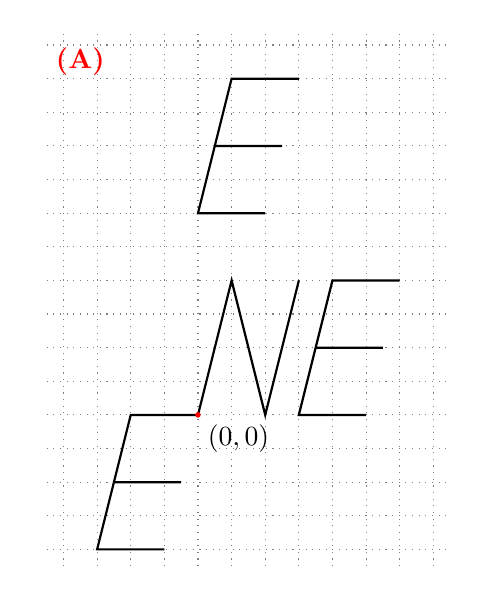
\begin{tikzpicture}
    \begin{axis}[scale=1.2,
		    axis equal image,
		    axis line style={draw=none},
		    tick style={draw=none},
		    yticklabels={,,},
		    xticklabels={,,},
		 xmin=-4.5,
		 xmax=7.5,
		 ymin=-4.5,
		 ymax=11.5,
		 major grid style={dotted, gray},
                 xtick={-10,-9,...,10},
                 ytick={-10,-9,...,11},
                 grid=both]
	\draw[black, thick] (0, 0) -- (1, 4) -- (2, 0) -- (3, 4);

	\draw[black, thick] (-1, -4) -- (-3, -4) -- (-2, 0) -- (0, 0)  (-2.5, -2) -- (-0.5, -2);
	\draw[black, thick] (5, 0) -- (3, 0) -- (4, 4) -- (6, 4) (3.5, 2) -- (5.5, 2);
	\draw[black, thick](2, 6) -- (0, 6) -- (1, 10) -- (3, 10) (0.5, 8) -- (2.5, 8) ;
	    \node[red] at (-3.5,10.5) {\bfseries (A)};
	    \fill[red] (0,0) circle[radius=1pt] node[below right, black] {$(0,0)$};
    \end{axis}
\end{tikzpicture}
\hfill
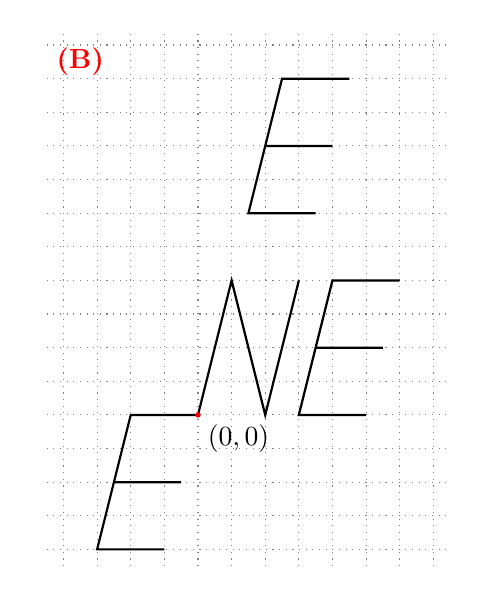
\begin{tikzpicture}
    \begin{axis}[scale=1.2,
		    axis equal image,
		    axis line style={draw=none},
		    tick style={draw=none},
		    yticklabels={,,},
		    xticklabels={,,},
		 xmin=-4.5,
		 xmax=7.5,
		 ymin=-4.5,
		 ymax=11.5,
		 major grid style={dotted, gray},
                 xtick={-10,-9,...,10},
                 ytick={-10,-9,...,11},
                 grid=both]
	\draw[black, thick] (0, 0) -- (1, 4) -- (2, 0) -- (3, 4);

	\draw[black, thick] (-1, -4) -- (-3, -4) -- (-2, 0) -- (0, 0)  (-2.5, -2) -- (-0.5, -2);
	\draw[black, thick] (5, 0) -- (3, 0) -- (4, 4) -- (6, 4) (3.5, 2) -- (5.5, 2);
	\draw[black, thick] (3.5, 6) -- (1.5, 6) -- (2.5, 10) -- (4.5, 10) (2.0, 8) -- (4.0, 8);
	    \node[red] at (-3.5,10.5) {\bfseries (B)};
	    \fill[red] (0,0) circle[radius=1pt] node[below right, black] {$(0,0)$};
    \end{axis}
\end{tikzpicture}
\end{minipage}
\hfill

\hfill
\begin{minipage}{6.5in}
	\hspace{2.13in}
	\hfill
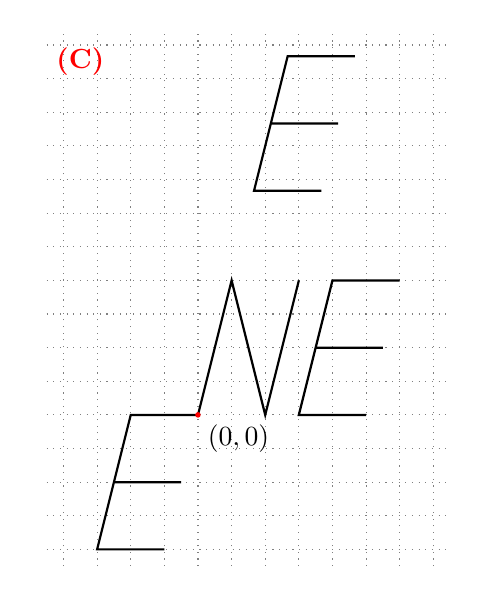
\begin{tikzpicture}
    \begin{axis}[scale=1.2,
		    axis equal image,
		    axis line style={draw=none},
		    tick style={draw=none},
		    yticklabels={,,},
		    xticklabels={,,},
		 xmin=-4.5,
		 xmax=7.5,
		 ymin=-4.5,
		 ymax=11.5,
		 major grid style={dotted, gray},
                 xtick={-10,-9,...,10},
                 ytick={-10,-9,...,11},
                 grid=both]
	\draw[black, thick] (0, 0) -- (1, 4) -- (2, 0) -- (3, 4);

	\draw[black, thick] (-1, -4) -- (-3, -4) -- (-2, 0) -- (0, 0)  (-2.5, -2) -- (-0.5, -2);
	\draw[black, thick] (5, 0) -- (3, 0) -- (4, 4) -- (6, 4) (3.5, 2) -- (5.5, 2);
	\draw[black, thick] (3.666666666666667, 6.666666666666667) -- (1.6666666666666667, 6.666666666666667) -- (2.666666666666667, 10.666666666666668) -- (4.666666666666667, 10.666666666666668)  (2.166666666666667, 8.666666666666668) -- (4.166666666666667, 8.666666666666668);
	    \node[red] at (-3.5,10.5) {\bfseries (C)};
	    \fill[red] (0,0) circle[radius=1pt,fill=blue] node[below right, black] {$(0,0)$};
    \end{axis}
\end{tikzpicture}
\hfill
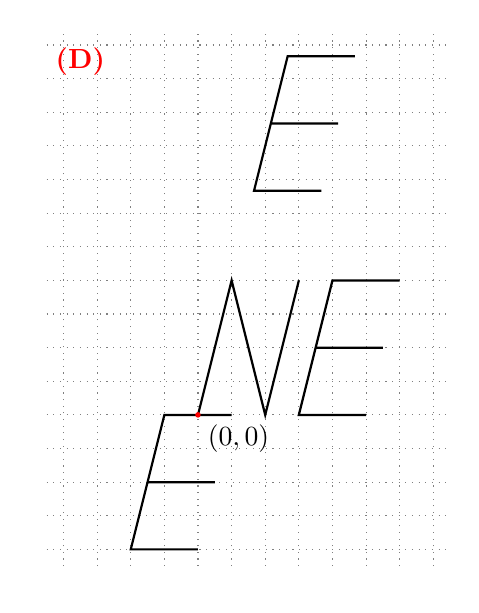
\begin{tikzpicture}
    \begin{axis}[scale=1.2,
		    axis equal image,
		    axis line style={draw=none},
		    tick style={draw=none},
		    yticklabels={,,},
		    xticklabels={,,},
		 xmin=-4.5,
		 xmax=7.5,
		 ymin=-4.5,
		 ymax=11.5,
		 major grid style={dotted, gray},
                 xtick={-10,-9,...,10},
                 ytick={-10,-9,...,11},
                 grid=both]
	\draw[black, thick] (0, 0) -- (1, 4) -- (2, 0) -- (3, 4);

	\draw[black, thick] (0, -4) -- (-2, -4) -- (-1, 0) -- (1, 0)  (-1.5, -2) -- (0.5, -2);
	\draw[black, thick] (5, 0) -- (3, 0) -- (4, 4) -- (6, 4) (3.5, 2) -- (5.5, 2);
	\draw[black, thick] (3.666666666666667, 6.666666666666667) -- (1.6666666666666667, 6.666666666666667) -- (2.666666666666667, 10.666666666666668) -- (4.666666666666667, 10.666666666666668)  (2.166666666666667, 8.666666666666668) -- (4.166666666666667, 8.666666666666668);
	    \node[red] at (-3.5,10.5) {\bfseries (D)};
	    \fill[red] (0,0) circle[radius=1pt,fill=blue] node[below right, black] {$(0,0)$};
    \end{axis}
\end{tikzpicture}
\end{minipage}
\hfill
\vfill







	\newpage
\pagestyle{siefken}
\section*{Linear Transformations}
\vspace{-1.5em}
	
	\question
	$\mathcal R:\R^2\to\R^2$ is the transformation that rotates vectors counter-clockwise 
	by $90^\circ$.
	\begin{parts}
		\item Compute $\mathcal R\mat{1\\0}$ and $\mathcal R\mat{0\\1}$.
		\item Compute $\mathcal R\mat{1\\1}$.  How does this relate to
			$\mathcal R\mat{1\\0}$ and $\mathcal R\mat{0\\1}$?
		\item What is $\mathcal R\left(a\mat{1\\0}+b\mat{0\\1}\right)$?
		\item Write down a matrix $R$ so that $R\vec v$ is $\vec v$ rotated
			counter clockwise by $90^\circ$.
	\end{parts}

	\begin{definition}[Linear Transformation]
		Let $V$ and $W$ be subspaces. A function $T:V\to W$ is called a \emph{linear transformation}
		if 
		\[
			T(\vec u+\vec v)=T\vec u+T\vec v \qquad\text{and}\qquad
			T(\alpha \vec v)=\alpha T\vec v
		\]
		for all vectors $\vec u,\vec v\in V$ and all scalars $\alpha$.
	\end{definition}

	\question
	\begin{parts}
		\item Classify the following as linear transformation or not
			\begin{enumerate}
				\item $\mathcal R$ from before (rotation counter-clockwise by $90^\circ$).
				\item $W:\R^2\to\R^2$ where $W\mat{x\\y}=\mat{x^2\\y}$.
				\item $T:\R^2\to\R^2$ where $T\mat{x\\y}=\mat{x+2\\y}$.
				\item $\mathcal P:\R^2\to\R^2$ where 
					$\mathcal P\mat{x\\y}=\Comp_{\vec u}\mat{x\\y}$ and 
					$\vec u=\mat{2\\3}$.
			\end{enumerate}
	\end{parts}

\begin{lesson}
	\newpage
	\Title{Linear Transformations II, Composition of Linear Transformations}

	\Heading{Textbook}
	Section 1.2

	\Heading{Objectives}
	\begin{itemize}
		\item 
	\end{itemize}

	\Heading{Motivation}

	\newpage
\end{lesson}
	\begin{definition}[Image of a Set]
		Let $L:V\to W$ be a transformation and let $X\subset V$ be a set.
		The \emph{image of the set $V$ under $L$}, denoted $L(V)$, is the set
		\[
			L(V)=\{\vec x: \vec x=L(\vec y)\text{ for some }\vec y\in V\}.
		\]
	\end{definition}

	\question
	Let $S=\{\mat{x\\y}:0\leq x,y\leq 1\}\subseteq \R^2$ be the filled-in unit square
	and let $C=\{\vec 0, \vec e_1,\vec e_2,\vec e_1+\vec e_2\}\subseteq \R^2$ be the corners of the 
	unit square.
	\begin{parts}
		\item Find $\mathcal R(C)$, $W(C)$, and $T(C)$ (where $\mathcal R$, $W$,
			and $T$ are from the previous question).
		\item Draw $\mathcal R(S)$, $T(S)$, and $\mathcal P(S)$ (where $\mathcal R$, $T$,
			and $\mathcal P$ are from the previous question).
		\item Suppose that $\ell=\{\text{ all convex combinations of }\vec a\text{ and }\vec b\}$
			is a line segment with endpoints $\vec a$ and $\vec b$
			and $A$ is a linear transformation. Must $A(\ell)$ be a line segment? What are
			its endpoints?
		\item Explain how images of sets relate to the \emph{Italicising N} task.
	\end{parts}

\newpage
\pagestyle{iola}
\section*{Task 2.3: Pat and Jamie}
\addcontentsline{toc}{subsection}{Task 2.3: Pat and Jamie}

\begin{minipage}{.5\textwidth}
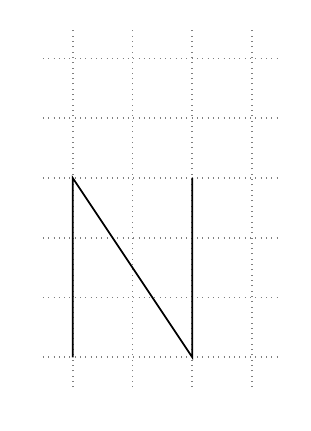
\begin{tikzpicture}[scale=.8]
    \begin{axis}[
		    axis equal image,
		    axis line style={draw=none},
		    tick style={draw=none},
		    yticklabels={,,},
		    xticklabels={,,},
		 xmin=-.5,
		 xmax=3.5,
		 ymin=-.5,
		 ymax=5.5,
		 major grid style={dotted, gray, thick},
                 xtick={0,1,2,3},
		 ytick={0,1,2,3,4,5},
                 grid=both]

	 \draw[black, thick] (0,0) -- (0,3) -- (2,0) -- (2,3);
    \end{axis}
\end{tikzpicture}\hfill
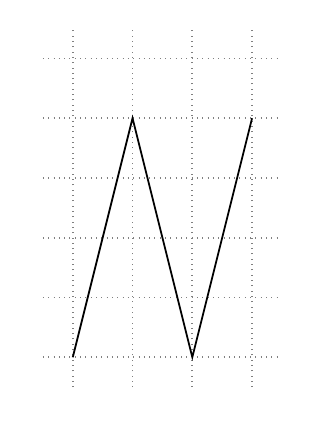
\begin{tikzpicture}[scale=.8]
    \begin{axis}[
		    axis equal image,
		    axis line style={draw=none},
		    tick style={draw=none},
		    yticklabels={,,},
		    xticklabels={,,},
		 xmin=-.5,
		 xmax=3.5,
		 ymin=-.5,
		 ymax=5.5,
		 major grid style={dotted, gray, thick},
                 xtick={0,1,2,3},
		 ytick={0,1,2,3,4,5},
                 grid=both]

	 \draw[black, thick] (0,0) -- (1,4) -- (2,0) -- (3,4);
    \end{axis}
\end{tikzpicture}\hfill
\end{minipage}
\begin{minipage}{.5\textwidth}

Suppose that the ``N'' on the left is written in regular 12-point font.  Find a matrix $A$ that will transform
	the ``N'' into the letter on the right which is written in an \emph{italic} 16-point font.
\end{minipage}

Two students---Pat and Jamie---explained their approach to the Italicizing N task as follows:
\begin{quote}\itshape
	In order to find the matrix $A$, we are going to find a matrix that makes the ``N'' taller,
	find a matrix that italicizes the taller ``N,'' and a combination of those two matrices
	will give the desired matrix $A$.
\end{quote}

\begin{enumerate}
	\item Do you think Pat and Jamie's approach allowed them to find $A$?  If so, do
		you think they found the same matrix that you did during Italicising N?
	\item Try Pat and Jamie's approach.  Either (a) come up with a matrix $A$ using
		their approach, or (b) explain why their approach does not work.
\end{enumerate}

\newpage
\pagestyle{siefken}


\begin{lesson}
	\newpage
	\Title{Range, Nullspace}

	\Heading{Textbook}
	Section 3.4

	\Heading{Objectives}
	\begin{itemize}
		\item 
	\end{itemize}

	\Heading{Motivation}

	\newpage
\end{lesson}
	\question
	Define $\mathcal P$ to be projection onto $\Span\{\vec u\}$ where $\vec u=\mat{2\\3}$,
	and let $\mathcal R$ be rotation counter-clockwise by $90^\circ$.
	\begin{parts}
		\item Find a matrix $P$ so that $P\vec x=\mathcal P(\vec x)$ for all $\vec x\in\R^2$.
		\item Find a matrix $R$ so that $R\vec x=\mathcal R(\vec x)$ for all $\vec x\in\R^2$.
		\item Write down matrices $A$ and $B$
			for $\mathcal P\circ\mathcal R$ and $\mathcal R\circ \mathcal P$.
		\item How do the matrices $A$ and $B$ relate to the matrices $P$ and $R$?
	\end{parts}

	\begin{definition}[Range]
		The \emph{range} (or \emph{image}) of a linear transformation $T:V\to W$ is the set of vectors that
		$T$ can output.  That is,
		\[
			\Range(T)=\{\vec y\in W:\vec y=T\vec x\text{ for some }\vec x\in V\}.
		\]
	\end{definition}
	\begin{definition}[Null Space]
		The \emph{null space} (or \emph{kernel}) of a linear transformation $T:V\to W$ is the
		set of vectors that get mapped to zero under $T$.  That is,
		\[
			\Null(T)=\{\vec x\in V:T\vec x=\vec 0\}.
		\]
	\end{definition}

	\question
	Let $\mathcal P:\R^2\to\R^2$ be projection onto $\Span\{\vec u\}$ where $\vec u=\mat{2\\3}$ (like before).
	\begin{parts}
		\item What is the range of $\mathcal P$?
		\item What is the null space of $\mathcal P$?
	\end{parts}

	\question
	Let $T:\R^n\to\R^m$ be an arbitrary linear transformation.
	\begin{parts}
		\item Show that the null space of $T$ is a subspace.
		\item Show that the range of $T$ is a subspace.
	\end{parts}

	\begin{definition}[Induced Transformation]
		Let $M$ be an $n\times m$ matrix. We say $M$ \emph{induces} 
		a linear transformation $T_M:\R^m\to\R^n$ defined by
		\[
			[T_M\vec v]_{\mathcal E'} = M[\vec v]_{\mathcal E},
		\]
		where $\mathcal E$ is the standard basis for $\R^m$ and $\mathcal E'$
		is the standard basis for $\R^n$.
	\end{definition}

\begin{lesson}
	\newpage
	\Title{Fundamental Subspaces}

	\Heading{Textbook}
	Section 3.4

	\Heading{Objectives}
	\begin{itemize}
		\item 
	\end{itemize}

	\Heading{Motivation}

	\newpage
\end{lesson}
	\question
	Let $M$ be a $2\times 2$ matrix and let $\vec v\in\R^2$. Further, let $T_M$
	be the transformation induced by $M$.
	\begin{parts}
		\item What is the difference between
			``$M\vec v$'' and $M[\vec v]_{\mathcal E}$''?
		\item What is $[T_M\vec e_1]_{\mathcal E}$?
		\item Can you relate the columns of $M$ to the range of $T_M$?
	\end{parts}


	\begin{definition}[Fundamental Subspaces]
		Associated with any matrix $M$ are three fundamental subspaces: the \emph{row space}
		of $M$ is the span of the rows of $M$; the \emph{column space} of $M$ is the span
		of the columns of $M$; and the \emph{null space} of $M$ is the set of solutions
		to $M\vec x=\vec 0$. 
		
	\end{definition}

	\question
	Consider $A=\mat{1&0&0\\0&1&0}$.
	\begin{parts}
		\item Describe the row space of $A$.
		\item Describe the column space of $A$.
		\item Is the row space of $A$ the same as the column space of $A$?
		\item Describe the set of all vectors perpendicular to the rows of $A$.
		\item Describe the null space of $A$.
		\item Describe the range and null space of $T_A$, the transformation induced
			by $A$.
	\end{parts}

	\question
	\[
		B=\mat{1&2&3\\1&1&1}\qquad C=\rref(B)=\mat{1&0&-1\\0&1&2}
	\]
	\begin{parts}
		\item How does the row space of $B$ relate to the row space of $C$?
		\item How does the null space of $B$ relate to the null space of $C$?
		\item Compute the null space of $B$.
	\end{parts}

	\question
	\[
		P=\mat{0&0\\1&2}\qquad Q=\rref(P)=\mat{1&2\\0&0}
	\]
	\begin{parts}
		\item How does the column space of $P$ relate to the column space of $Q$?
		\item Describe the column space of $P$ and the column space of $Q$.
	\end{parts}


\begin{lesson}
	\newpage
	\Title{Rank}

	\Heading{Textbook}
	Section 3.4

	\Heading{Objectives}
	\begin{itemize}
		\item 
	\end{itemize}

	\Heading{Motivation}

	\newpage
\end{lesson}
	\newpage
	\begin{definition}[Rank]
		For a linear transformation $T:V\to W$, the \emph{rank} of $T$,
		denoted $\Rank(T)$, is the dimension of the range of $T$.

		For an $n\times m$ matrix $M$, the \emph{rank} of $M$, denoted
		$\Rank(M)$, is the number of pivots in $\rref(M)$.
	\end{definition}

	\question
	Let $\mathcal P$ be projection onto $\Span\{\vec u\}$ where $\vec u=\mat{2\\3}$,
	and let $\mathcal R$ be rotation counter-clockwise by $90^\circ$.
	\begin{parts}
		\item Describe $\Range(\mathcal P)$ and $\Range(\mathcal R)$.
		\item What is the rank of $\mathcal P$ and the rank of $\mathcal R$?
		\item Let $P$ and $R$ be the matrices corresponding to $\mathcal P$ and
			$\mathcal R$. What is the rank of $P$ and the rank of $R$?
		\item Make a conjecture about how the rank of a transformation and
			the rank of its corresponding matrix relate. Can you justify your claim?
	\end{parts}


	\question
	\begin{parts}
		\item Determine the rank of
		\begin{enumerate*}
			\item $\mat{1&1\\2&2}$
			\item $\mat{1&2\\3&4}$
			\item $\mat{1&1&0\\0&0&1}$
			\item $\mat{3\\3\\2}$
			\item $\mat{1&0&1\\0&1&0\\0&0&1}$.
		\end{enumerate*}
	\end{parts}
	
	\question
	Consider the homogeneous system 
		\begin{equation}\label{eq4b}
			\begin{array}{llll}
				x&+2y&+z &= 0\\
				x&+2y&+3z &= 0\\
				-x&-2y&+z &= 0
			\end{array}
		\end{equation}
	and the non-augmented matrix of coefficients $A=\mat{1&2&1\\1&2&3\\-1&-2&1}$.
	\begin{parts}
		\item What is $\Rank(A)$?
		\item Give the general solution to \eqref{eq4b}.
		\item Are the column vectors of $A$ linearly independent?
		\item Give a non-homogeneous system with the same coefficients as \eqref{eq4b} that has
			\begin{enumerate}
				\item infinitely many solutions
				\item no solutions.
			\end{enumerate}
	\end{parts}

	\question
	\begin{parts}
		\item The rank of a $3\times 4$ matrix $A$ is $3$.  Are the column vectors of $A$ linearly independent?
		\item The rank of a $4\times 3$ matrix $B$ is $3$.  Are the column vectors of $B$ linearly independent?
	\end{parts}


\begin{lesson}
	\newpage
	\Title{Rank-nullity Theorem, Inverses I}

	\Heading{Textbook}
	Section 1.2

	\Heading{Objectives}
	\begin{itemize}
		\item 
	\end{itemize}

	\Heading{Motivation}

	\newpage
\end{lesson}
	\begin{theorem}[Rank-nullity Theorem]
	The \emph{nullity} of a matrix is the dimension of the null space.

	The rank-nullity theorem for a matrix $A$ states
	\[
		\rank(A)+\nnul(A) = \#\text{ of columns in }A.
	\]
	\end{theorem}

	\question
	\begin{parts}
		\item Is here a version of the rank-nullity theorem that applies to linear
			transformations instead of matrices? If so, state it.
	\end{parts}

	\question
	The vectors $\vec u,\vec v\in\R^9$ are linearly independent and $\vec w=2\vec u-\vec v$.
	Define $A=[\vec u|\vec v|\vec w]$.
	\begin{parts}
		\item What is the rank and nullity of $A^T$?
		\item What is the rank and nullity of $A$?
	\end{parts}









\newpage
\pagestyle{iola}
\section*{Task 2.4: Getting back N}
\addcontentsline{toc}{subsection}{Task 2.4: Getting back N}

\begin{minipage}{.5\textwidth}
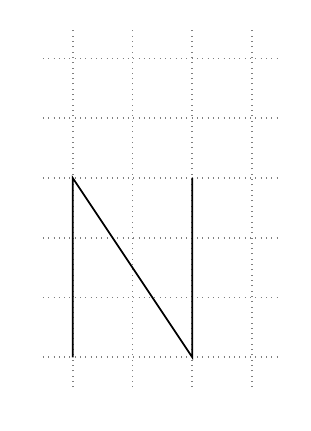
\begin{tikzpicture}[scale=.8]
    \begin{axis}[
		    axis equal image,
		    axis line style={draw=none},
		    tick style={draw=none},
		    yticklabels={,,},
		    xticklabels={,,},
		 xmin=-.5,
		 xmax=3.5,
		 ymin=-.5,
		 ymax=5.5,
		 major grid style={dotted, gray, thick},
                 xtick={0,1,2,3},
		 ytick={0,1,2,3,4,5},
                 grid=both]

	 \draw[black, thick] (0,0) -- (0,3) -- (2,0) -- (2,3);
    \end{axis}
\end{tikzpicture}\hfill
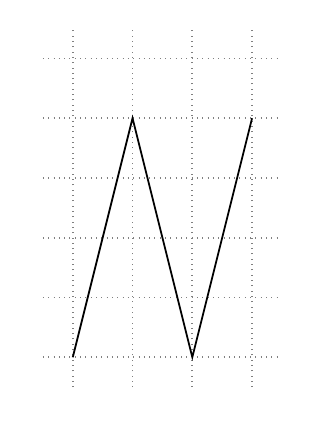
\begin{tikzpicture}[scale=.8]
    \begin{axis}[
		    axis equal image,
		    axis line style={draw=none},
		    tick style={draw=none},
		    yticklabels={,,},
		    xticklabels={,,},
		 xmin=-.5,
		 xmax=3.5,
		 ymin=-.5,
		 ymax=5.5,
		 major grid style={dotted, gray, thick},
                 xtick={0,1,2,3},
		 ytick={0,1,2,3,4,5},
                 grid=both]

	 \draw[black, thick] (0,0) -- (1,4) -- (2,0) -- (3,4);
    \end{axis}
\end{tikzpicture}\hfill
\end{minipage}
\begin{minipage}{.5\textwidth}

Suppose that the ``N'' on the left is written in regular 12-point font.  Find a matrix $A$ that will transform
	the ``N'' into the letter on the right which is written in an \emph{italic} 16-point font.
\end{minipage}

Two students---Pat and Jamie---explained their approach to the Italicizing N task as follows:
\begin{quote}\itshape
	In order to find the matrix $A$, we are going to find a matrix that makes the ``N'' taller,
	find a matrix that italicizes the taller ``N,'' and a combination of those two matrices
	will give the desired matrix $A$.
\end{quote}

Consider the new task: find a matrix $C$ that transforms the ``N'' on the right to
the ``N'' on the left.
\begin{enumerate}
	\item Use any method you like to find $C$.
	\item Use a method similar to Pat and Jamie's method, only use it to find $C$ instead
		of $A$.
\end{enumerate}


\newpage
\pagestyle{siefken}

\begin{lesson}
	\newpage
	\Title{Inverses II, Elementary Matrices}

	\Heading{Textbook}
	Section 3.5

	\Heading{Objectives}
	\begin{itemize}
		\item 
	\end{itemize}

	\Heading{Motivation}

	\newpage
\end{lesson}

\section*{Inverses}

	\question
	\begin{parts}
		\item Apply the row operation $R_3\to R_3+2R_1$ to the $3\times 3$ identity
		matrix and call the result $E_1$.
		\item Apply the row operation $R_3\to R_3-2R_1$ to the $3\times 3$ identity
		matrix and call the result $E_2$.
	\end{parts}

	\begin{definition}
	An \emph{elementary matrix} is the identity matrix with a single row operation applied.
	\end{definition}

	\[
		A=\mat{1&2&3\\4&5&6\\7&8&9}
	\]
	\begin{parts}[resume]
		\item Compute $E_1A$ and $E_2A$.  How do the resulting matrices relate to row
		operations?
		\item Without computing, what should the result of applying the row
		operation $R_3\to R_3-2R_1$ to $E_1$ be?  Compute and verify.
		\item Without computing, what should $E_1E_2$ be?  What about $E_2E_1$?
		Now compute and verify.
	\end{parts}

	\begin{definition}
		The \emph{inverse} of a matrix $A$ is a
		matrix $B$ such that $AB=I$ and $BA=I$.
		In this case, $B$ is called the inverse of $A$ and is notated by $A^{-1}$.
	\end{definition}

	\question
	Consider the matrices 
	\[
		A=\mat{1&2&0\\0&1&0\\-3&-6&1}\qquad
		B=\mat{1&0&0\\0&1&0}\qquad
		C=\mat{1&0\\0&1\\0&0}
	\]
	\[
		D=\mat{1&-2&0\\0&1&0\\3&0&1}\qquad
		E=\mat{1&0&0\\0&2&0\\0&1&1}\qquad
		F=\mat{1&0&0\\0&1&0\\0&0&1}
	\]
	\begin{parts}
		\item Which pairs of matrices above are inverses of each other?
	\end{parts}

	\question
	\[
		B=\mat{1 &4\\0 &2}
	\]
	\begin{parts}
		\item Use two row operations to reduce $B$ to $I_{2\times 2}$
		and write an elementary matrix $E_1$ corresponding to the first operation
		and $E_2$ corresponding to the second.
		\item What is $E_2E_1B$?
		\item Find $B^{-1}$.
		\item Can you outline a procedure for finding the inverse of a matrix
		using elementary matrices?
	\end{parts}

\begin{lesson}
	\newpage
	\Title{Applications of Inverses I}

	\Heading{Textbook}
	Section 3.5

	\Heading{Objectives}
	\begin{itemize}
		\item 
	\end{itemize}

	\Heading{Motivation}

	\newpage
\end{lesson}
	\question
	\[
		A=\mat{1&2&-1\\2&2&4\\1&3&-3}\qquad
		\vec b=\mat{1\\2\\3}\qquad
		C=[A|\vec b]\qquad
		A^{-1}=\mat{9&-3/2&-5\\-5&1&3\\-2&1/2&1}
	\]
	\begin{parts}
		\item What is $A^{-1}A$?
		\item What is $\rref(A)$?
		\item What is $\rref(C)$? (Hint, there is no need to actually do row reduction!)
		\item Solve the system $A\vec x=\vec b$.
	\end{parts}

	\question
	\begin{parts}
		\item For two square matrices $X,Y$, should $(XY)^{-1}=X^{-1}Y^{-1}$?
		\item If $M$ is a matrix corresponding to a non-invertible linear transformation $T$,
			could $M$ be invertible?
	\end{parts}

\subsection*{More Change of Basis}
	\question
	Let $\mathcal B=\{\vec b_1,\vec b_2\}$ where $\vec b_1=\mat{1\\1}$, $\vec b_2=\mat{1\\-1}$
	and let $X=[\vec b_1|\vec b_2]$ be the matrix whose columns are $\vec b_1$ and $\vec b_2$.
	\begin{parts}
		\item Compute $[\vec e_1]_{\mathcal B}$ and $[\vec e_2]_{\mathcal B}$.
		\item Compute $X[\vec e_1]_{\mathcal B}$ and $X[\vec e_2]_{\mathcal B}$.  
			What do you notice?
		\item Find the matrix $X^{-1}$. How does $X^{-1}$ relate to change of basis?
	\end{parts}

	
\begin{lesson}
	\newpage
	\Title{Applications of Inverses II, Change of Basis}

	\Heading{Textbook}
	Section 4.4

	\Heading{Objectives}
	\begin{itemize}
		\item 
	\end{itemize}

	\Heading{Motivation}

	\newpage
\end{lesson}
	\question
	Let $\mathcal S=\{\vec e_1,\vec e_2,\ldots,\vec e_n\}$ be the standard basis for $\R^n$.
	Given a basis $\mathcal B=\{\vec b_1,\vec b_2,\ldots,\vec b_n\}$ for $\R^n$, the 
	matrix $X=[\vec b_1|\vec b_2|\cdots|\vec b_n]$ converts
	vectors from the $\mathcal B$ basis into the standard basis.  In other words,
	\[
		X[\vec v]_{\mathcal B} = [\vec v]_{\mathcal S}.
	\]
	\begin{parts}
		\item Should $X^{-1}$ exist? Explain.
		\item Consider the equation\[
				X^{-1}[\vec v]_{?} = [\vec v]_{?}.
			\]
			Can you fill in the ``?''~symbols so that the equation makes sense?
		\item What is $[\vec b_1]_{\mathcal B}$?  How about $[\vec b_2]_{\mathcal B}$?  Can
			you generalize to $[\vec b_i]_{\mathcal B}$?
	\end{parts}

	\question
	Let $\vec c_1=\mat{2\\1}$, $\vec c_2=\mat{5\\3}$, $\mathcal C=\{\vec c_1,\vec c_2\}$, and $A=\mat{2&5\\1&3}$.
	Note that $A^{-1}=\mat{3&-5\\-1&2}$ and that $A$ changes vectors from the $\mathcal C$ basis to the standard
	basis and $A^{-1}$ changes vectors from the standard basis to the $\mathcal C$ basis.
	\begin{parts}
		\item Compute $[\vec c_1]_{\mathcal C}$ and $[\vec c_2]_{\mathcal C}$.
	\end{parts}
	Let $T:\R^2\to\R^2$ be the linear transformation that stretches in the $\vec c_1$ direction by a factor of $2$
	and doesn't stretch in the $\vec c_2$ direction at all.
	\begin{parts}[resume]
		\item Compute $T\mat{2\\1}$ and $T\mat{5\\3}$.
		\item Compute $[T\vec c_1]_{\mathcal C}$ and $[T\vec c_2]_{\mathcal C}$.
		\item Compute the result of $T\mat{\alpha\\\beta}_{\mathcal C}$ and express the result in the
			$\mathcal C$ basis (i.e., as a vector of the form $\mat{?\\?}_{\mathcal C}$).
		\item Find $[T]_{\mathcal C}$, the matrix for $T$ in the $\mathcal C$ basis.
		\item Find $[T]_{\mathcal E}$, the matrix for $T$ in the standard basis.
	\end{parts}
	\begin{definition}[Similar Matrices]
		A matrices $A$ and $B$ are called \emph{similar matrices}, denoted $A\sim B$, if
		$A$ and $B$ represent the same linear transformation but in possibly different bases.
		Equivalently, $A\sim B$ if there is an invertible matrix $X$ so that
		\[
			A=XBX^{-1}.
		\]
	\end{definition}



	
\begin{lesson}
	\newpage
	\Title{Determinants}

	\Heading{Textbook}
	Section 5.4

	\Heading{Objectives}
	\begin{itemize}
		\item 
	\end{itemize}

	\Heading{Motivation}

	\newpage
\end{lesson}
\newpage
\section*{Determinants}
	\begin{definition}[Unit $n$-cube]
		The unit $n$-cube is the $n$-dimensional cube with side length 1 and lower-left
		corner located at the origin.  That is 
		\[
			C_n = \left\{\vec x\in\R^n:\vec x=\sum_{i=1}^n \alpha_i\vec e_i\text{ for some }\alpha_1,\ldots,\alpha_n\in[0,1]\right\}=[0,1]^n.
		\]
	\end{definition}
	The volume of the unit $n$-cube is always 1.

	\question
	The picture shows what the linear transformation $T$ does to the unit square (i.e., the unit $2$-cube).

	\begin{center}
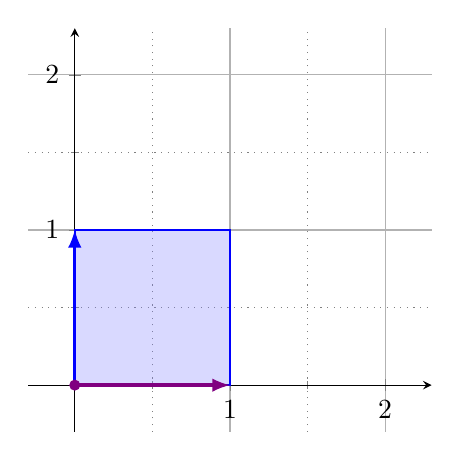
\begin{tikzpicture}[>=latex]
    \begin{axis}[scale=.9,
		    axis equal image,
		    axis lines=middle,
		    %axis line style={draw=none},
		    %tick style={draw=none},
		    %yticklabels={,,},
		    %xticklabels={,,},
		 xmin=-.3,
		 xmax=2.3,
		 ymin=-.3,
		 ymax=2.3,
		 major grid style={black!30!white},
		 minor grid style={dotted, gray},
		 minor tick num=1,
                 xtick={-10,-9,...,10},
                 ytick={-10,-9,...,10},
                 grid=both]



		\fill[blue!50!white, opacity=0.3] (0,0) -- (0,1) -- (1,1) -- (1,0) -- (0,0);
		\draw[thick,blue] (0,0) -- (0,1) -- (1,1) -- (1,0) -- (0,0);
		\draw[->,very thick,violet] (0,0) -- (1,0);
		\draw[->,very thick,blue] (0,0) -- (0,1);
	    \fill[fill=violet] (0,0) circle[radius=2pt];
    \end{axis}
\end{tikzpicture}\hspace{.5cm}
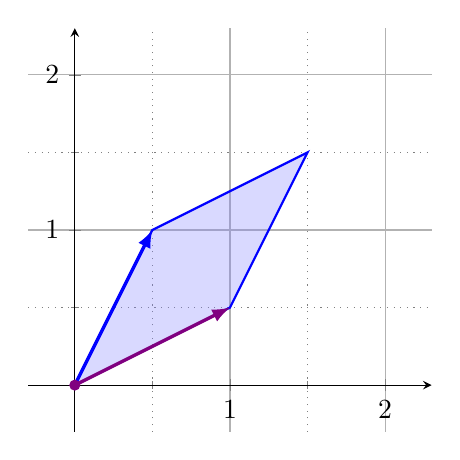
\begin{tikzpicture}[>=latex]
    \begin{axis}[scale=.9,
		    axis equal image,
		    axis lines=middle,
		    %axis line style={draw=none},
		    %tick style={draw=none},
		    %yticklabels={,,},
		    %xticklabels={,,},
		 xmin=-.3,
		 xmax=2.3,
		 ymin=-.3,
		 ymax=2.3,
		 major grid style={black!30!white},
		 minor grid style={dotted, gray},
		 minor tick num=1,
                 xtick={-10,-9,...,10},
                 ytick={-10,-9,...,10},
                 grid=both]



		\fill[blue!50!white, opacity=0.3] (0,0) -- (0.5,1) -- (1.5,1.5) -- (1,0.5) -- (0,0);
		\draw[thick,blue] (0,0) -- (0.5,1) -- (1.5,1.5) -- (1,0.5) -- (0,0);
		\draw[->,very thick,violet] (0,0) -- (1,0.5);
		\draw[->,very thick,blue] (0,0) -- (0.5,1);
	    \fill[fill=violet] (0,0) circle[radius=2pt];
    \end{axis}
\end{tikzpicture}
\end{center}


	\begin{parts}
		\item What is $T\mat{1\\0}$, $T\mat{0\\1}$, $T\mat{1\\1}$?
		\item Write down a matrix for $T$.
		\item What is the volume of the image of the unit square (i.e., the volume of $T(C_2)$)?  You may need
			to use trigonometry.
	\end{parts}
	
	\begin{definition}[Determinant]
	The \emph{determinant} of a linear transformation $X:\R^n\to \R^n$ is the 
	oriented volume of the image of the unit $n$-cube.  The determinant
	of a square matrix is the oriented volume of the parallelepiped 
		($n$-dimensional parallelogram) given by the column vectors (or the row
		vectors).
	\end{definition}

	\question
	We know the following about the transformation $A$:
	\[
		A\mat{1\\0}=\mat{2\\0}\qquad\text{and}\qquad A\mat{0\\1}=\mat{1\\1}.
	\]
	\begin{parts}
	\item Draw $C_2$ and $A(C_2)$, the image of the unit square
			under $A$.
		\item Compute the area of $A (C_2)$.
		\item Compute $\det(A)$.
	\end{parts}

	\question
	Suppose $R$ is a rotation counterclockwise by $30^\circ$.
	\begin{parts}
	\item Draw $C_2$ and $R(C_2)$.
	\item Compute the area of $R(C_2)$.
		\item Compute $\det(R)$.
	\end{parts}
	
	\question
	We know the following about the transformation $F$:
	\[
		F\mat{1\\0}=\mat{0\\1}\qquad\text{and}\qquad F\mat{0\\1}=\mat{1\\0}.
	\]
	\begin{parts}
		\item What is $\det(F)$?
	\end{parts}

\begin{lesson}
	\newpage
	\Title{Determinants and Compositions}

	\Heading{Textbook}
	Section 5.2

	\Heading{Objectives}
	\begin{itemize}
		\item 
	\end{itemize}

	\Heading{Motivation}

	\newpage
\end{lesson}
	\question
	Let $D=\{\vec x:\|\vec x\|\leq 1\}$ be the unit disk. You know the following about the 
	linear transformations $M$, $T$, and $S$: $M$ is
	defined by $\vec x\mapsto 2\vec x$; $T$ has determinant $2$; and $S$ has determinant $3$.
	\begin{parts}
		\item Find the oriented volumes of $M(C_2)$, $T(C_2)$, and $S(C_2)$.
		\item How does the volume of $T(C_2+\{\vec e_1\})$ compare to the volume 
			of $T(C_2)$?
		\item What is the oriented volume of $T\circ M(C_2)$? What is $\det(T\circ M)$?
		\item What is the oriented volume of $S(D)$?
	\end{parts}

	\question
	\begin{itemize}
		\item $E_f$ is $I_{3\times 3}$ with the first two rows swapped.
		\item $E_m$ is $I_{3\times 3}$ with the third row multiplied by 6.
		\item $E_a$ is $I_{3\times 3}$ with $R_1\to R_1+2R_2$ applied.
	\end{itemize}

	\begin{parts}
		\item What is $\det(E_f)$?
		\item What is $\det(E_m)$?
		\item What is $\det(E_a)$?
		\item What is $\det(E_fE_m)$?
		\item What is $\det(4I_{3\times 3})$?
		\item What is $\det(W)$ where $W=E_fE_aE_fE_mE_m$?
	\end{parts}

	\question
	$U=\mat{1&2&1&2\\0&3&-2&4\\0&0&-1&0\\0&0&0&4}$
	\begin{parts}
		\item What is $\det(U)$?
		\item $V$ is a square matrix and rref$(V)$ has a row of zeros.
		 What is $\det(V)$?
		\item $P$ is projection onto the vector $\mat{-1\\-1}$. What is $\det(P)$?
	\end{parts}

	\question
	Suppose you know $\det(X)=4$.
	\begin{parts}
		\item What is $\det(X^{-1})$?
		\item Derive a relationship between $\det(Y)$
			and $\det(Y^{-1})$ for an arbitrary matrix $Y$.
		\item Suppose $Y$ is not invertible.  What is $\det(Y)$?
	\end{parts}

\newpage
\pagestyle{iola}

\begin{lesson}
	\newpage
	\Title{Eigenstuff I}

	\Heading{Textbook}
	Section 6.1

	\Heading{Objectives}
	\begin{itemize}
		\item 
	\end{itemize}

	\Heading{Motivation}

	\newpage
\end{lesson}
\section*{Task 3.1: The Green and the Black}
\addcontentsline{toc}{subsection}{Task 3.1: The Green and the Black}
Consider the following two bases for $\R^2$: the green basis $\mathcal G=\{\vec g_1,\vec g_2\}$
and the black basis $\mathcal B=\{\vec e_1,\vec e_2\}$.
\begin{center}
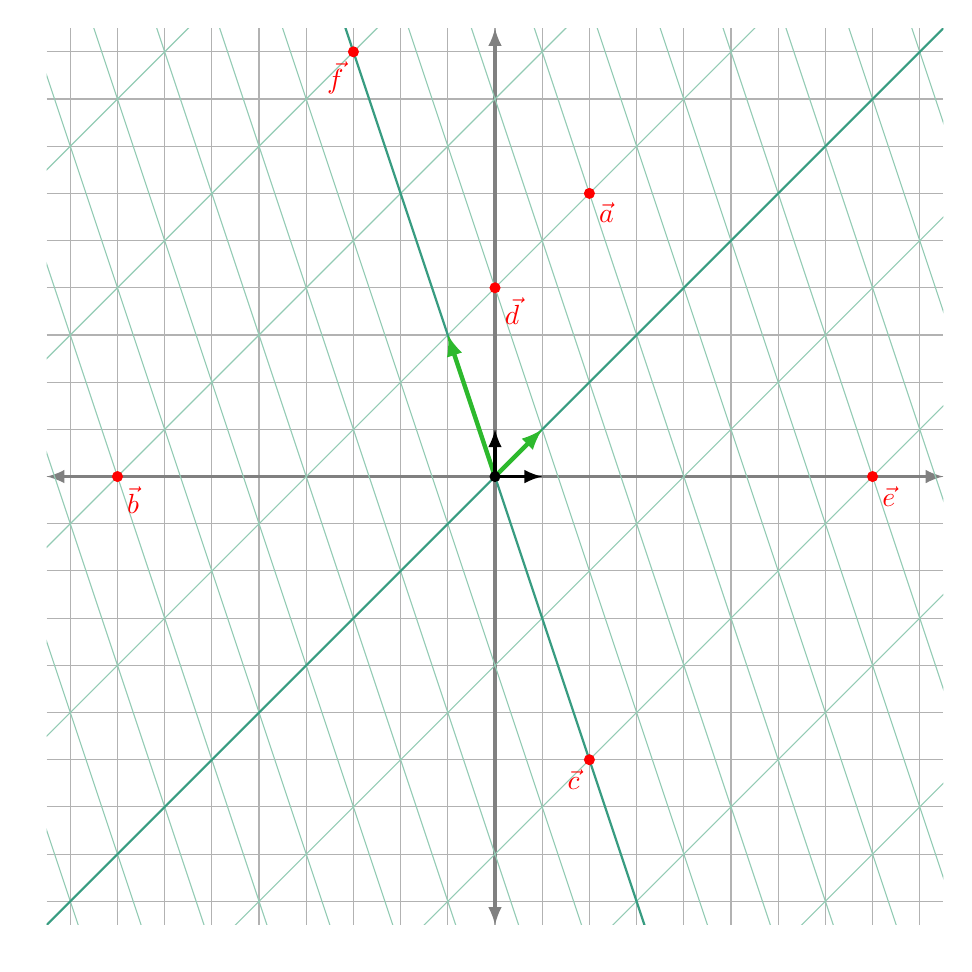
\begin{tikzpicture}[>=latex]
    \begin{axis}[scale=2,
		    axis equal image,
		    axis line style={draw=none},
		    tick style={draw=none},
		    yticklabels={,,},
		    xticklabels={,,},
		 xmin=-9.5,
		 xmax=9.5,
		 ymin=-9.5,
		 ymax=9.5,
		 major grid style={black!30!white},
                 xtick={-10,-9,...,11},
                 ytick={-10,-9,...,11},
                 grid=both]

		 \coordinate (A) at (-9.5, 0);
		 \coordinate (B) at (9.5, 0);
		 \coordinate (C) at (0, -9.5);
		 \coordinate (D) at (0, 9.5);
		\draw[<->, very thick, black!50!white] (A) -- (B);
		\draw[<->, very thick, black!50!white] (C) -- (D);
		

	    \foreach \ival in {-40,-36,...,40} {
	    	\edef\temp{\noexpand\draw[PineGreen!40!white] (-12,36+\ival) -- (12,-36+\ival);}
		\temp
	    	\edef\temp{\noexpand\draw[PineGreen!40!white] (-36,-36+\ival) -- (36,36+\ival);}
		\temp
	    }
	    \draw[PineGreen!80!white, thick] (-12,36) -- (12,-36) (-36,-36) -- (36, 36);
	    \draw[->, ultra thick, LimeGreen!90!black] (0,0) -- (1,1);
	    \draw[->, ultra thick, LimeGreen!90!black] (0,0) -- (-1,3);
	    \draw[->, very thick, black] (0,0) -- (0,1);
	    \draw[->, very thick, black] (0,0) -- (1,0);


	  	\fill[fill=black] (0,0) circle[radius=2pt];
	  	\fill[red] (2,6) circle[radius=2pt] node[below right] {$\vec a$};
	  	\fill[red] (-8,0) circle[radius=2pt] node[below right] {$\vec b$};
	  	\fill[red] (2,-6) circle[radius=2pt] node[below left] {$\vec c$};
	  	\fill[red] (0,4) circle[radius=2pt] node[below right] {$\vec d$};
	  	\fill[red] (8,0) circle[radius=2pt] node[below right] {$\vec e$};
	  	\fill[red] (-3,9) circle[radius=2pt] node[below left] {$\vec f$};
    \end{axis}
\end{tikzpicture}
\end{center}



\begin{enumerate}
	\item Write each point above in both the green and the black bases.
	\item Find a change-of-basis matrix $X$ that converts vectors from
		a green basis representation to a black basis representation. Find
		another matrix $Y$ that converts vectors from a black basis representation
		to a green basis representation.
	\item Let $T:\R^2\to\R^2$ be the linear transformation that stretches in the $y=-3x$ direction
		by a factor of $2$ and leaves vectors in the $y=x$ direction fixed.

		Describe what happens to the vectors $\vec u$, $\vec v$, and $\vec w$ when
		$T$ is applied given that 
		\[
			[\vec u]_{\mathcal G} = \mat{6\\1} \qquad 
			[\vec v]_{\mathcal G} = \mat{4\\-3} \qquad 
			[\vec u]_{\mathcal B} = \mat{-8\\-7}.
		\]
	\item When working with the transformation $T$, which basis do you prefer vectors be
		represented in?
\end{enumerate}




\newpage
\pagestyle{siefken}

\begin{lesson}
	\newpage
	\Title{Eigenstuff II}

	\Heading{Textbook}
	Section 6.1

	\Heading{Objectives}
	\begin{itemize}
		\item 
	\end{itemize}

	\Heading{Motivation}

	\newpage
\end{lesson}
\section*{Eigenvectors}

	\vspace{-.6cm}
	\begin{definition}[Eigenvector]
	Let $X$ be a linear transformation.  An \emph{eigenvector} for $X$ is a non-zero vector that doesn't
	change directions when $X$ is applied.  That is, $\vec v\neq \vec 0$ is an eigenvector for $X$ if
	\[
		X\vec v=\lambda \vec v
	\]
	for some scalar $\lambda$.  We call $\lambda$ the \emph{eigenvalue} 
	of $X$ corresponding
	to the eigenvector $\vec v$.
	\end{definition}
	\vspace{-.2cm}

	\question
	The picture shows what the linear transformation $T$ does to the unit square (i.e., the unit $2$-cube).

	\begin{center}
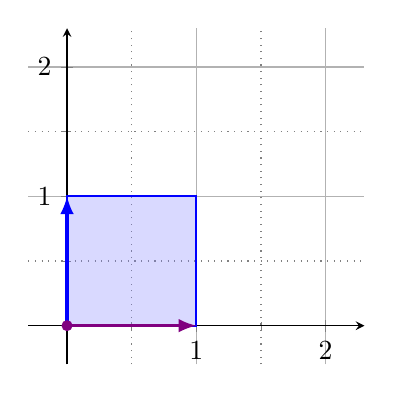
\begin{tikzpicture}[>=latex]
    \begin{axis}[scale=.75,
		    axis equal image,
		    axis lines=middle,
		    %axis line style={draw=none},
		    %tick style={draw=none},
		    %yticklabels={,,},
		    %xticklabels={,,},
		 xmin=-.3,
		 xmax=2.3,
		 ymin=-.3,
		 ymax=2.3,
		 major grid style={black!30!white},
		 minor grid style={dotted, gray},
		 minor tick num=1,
                 xtick={-10,-9,...,10},
                 ytick={-10,-9,...,10},
                 grid=both]



		\fill[blue!50!white, opacity=0.3] (0,0) -- (0,1) -- (1,1) -- (1,0) -- (0,0);
		\draw[thick,blue] (0,0) -- (0,1) -- (1,1) -- (1,0) -- (0,0);
		\draw[->,very thick,violet] (0,0) -- (1,0);
		\draw[->,very thick,blue] (0,0) -- (0,1);
	    \fill[fill=violet] (0,0) circle[radius=2pt];
    \end{axis}
\end{tikzpicture}\hspace{.5cm}
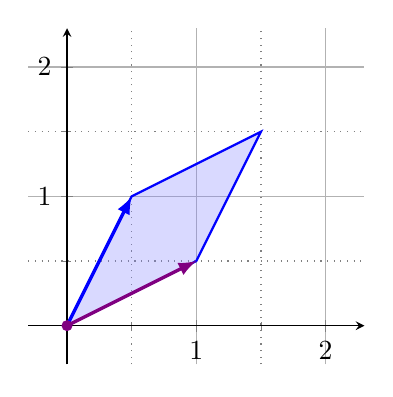
\begin{tikzpicture}[>=latex]
    \begin{axis}[scale=.75,
		    axis equal image,
		    axis lines=middle,
		    %axis line style={draw=none},
		    %tick style={draw=none},
		    %yticklabels={,,},
		    %xticklabels={,,},
		 xmin=-.3,
		 xmax=2.3,
		 ymin=-.3,
		 ymax=2.3,
		 major grid style={black!30!white},
		 minor grid style={dotted, gray},
		 minor tick num=1,
                 xtick={-10,-9,...,10},
                 ytick={-10,-9,...,10},
                 grid=both]



		\fill[blue!50!white, opacity=0.3] (0,0) -- (0.5,1) -- (1.5,1.5) -- (1,0.5) -- (0,0);
		\draw[thick,blue] (0,0) -- (0.5,1) -- (1.5,1.5) -- (1,0.5) -- (0,0);
		\draw[->,very thick,violet] (0,0) -- (1,0.5);
		\draw[->,very thick,blue] (0,0) -- (0.5,1);
	    \fill[fill=violet] (0,0) circle[radius=2pt];
    \end{axis}
\end{tikzpicture}
\end{center}
	

	\begin{parts}
		\item Give an eigenvector for $T$.  What is the eigenvalue?
		\item Can you give another?
	\end{parts}


	\question
	For some matrix $A$,
	\vspace{-.2cm}
	\[
		A\mat{3\\3\\1}=\mat{2\\2\\2/3}\qquad\text{ and }\qquad B=A-\tfrac{2}{3}I.
	\]
	\vspace{-.4cm}
	\begin{parts}
		\item Give an eigenvector and a corresponding eigenvalue for $A$.
		\item What is $B\mat{3\\3\\1}$?
		\item What is the dimension of $\text{null}(B)$?
		\item What is $\det(B)$?
	\end{parts}

	\vspace{-.2cm}
	\question
	Let $C=\mat{-1&2\\1&0}$ and $E_\lambda = C-\lambda I$.
	\begin{parts}
		\item For what values of $\lambda$ does $E_\lambda$ have a non-trivial
			null space?
		\item What are the eigenvalues of $C$?
		\item Find the eigenvectors of $C$.
	\end{parts}
	
\begin{lesson}
	\newpage
	\Title{Characteristic Polynomial, Diagonalization I}

	\Heading{Textbook}
	Section 6.2

	\Heading{Objectives}
	\begin{itemize}
		\item 
	\end{itemize}

	\Heading{Motivation}

	\newpage
\end{lesson}
	\begin{definition}[Characteristic Polynomial]
	For a matrix $A$, the \emph{characteristic polynomial} of $A$ is
	\[
		\chr(A)=\det(A-\lambda I).
	\]
	\end{definition}
	\vspace{-.4cm}
	
	\question
	Let $D=\mat{1&2\\3&0}$.
	\begin{parts}
		\item Compute $\chr(D)$.
		\item Find the eigenvalues of $D$.
	\end{parts}

	\vspace{-.3cm}
	\question
	\vspace{-.2cm}
	Suppose $\chr(E)=\lambda(\lambda -2)(\lambda +3)$ for some unknown $3\times 3$
	matrix $E$.
	\begin{parts}
		\item What are the eigenvalues of $E$?
		\item Is $E$ invertible?
		\item What is $\nnul(E)$, $\nnul(E-3I)$, $\nnul(E+3I)$?
	\end{parts}

	\question
	Consider
	\[
		A=\mat{1&0&1\\0&1&1\\1&1&0}\qquad
		\vec v_1=\mat{1\\1\\1}\qquad
		\vec v_2=\mat{1\\1\\-2}\qquad
		\vec v_3=\mat{-1\\1\\0}
	\]
	and notice that $\vec v_1,\vec v_2,\vec v_3$ are eigenvectors for $A$.
	\begin{parts}
		\item Find the eigenvalues of $A$.
		\item Find the characteristic polynomial of $A$.
		\item Compute $A\vec w$ where $w=2\vec v_1-\vec v_2$.
		\item Compute $A\vec u$ where $\vec u=a\vec v_1+b\vec v_2+c\vec v_3$ for
			unknown scalar coefficients $a,b,c$.
	\end{parts}
	Notice that $\mathcal V=\{\vec v_1,\vec v_2,\vec v_3\}$ is a basis for $\R^3$.
	\begin{parts}[resume]
	\item If $[\vec x]_{\mathcal V}=\mat{1\\3\\4}$ is $\vec x$ written in the $\mathcal V$ basis,
		compute $A\vec x$ in the $\mathcal V$ basis.
	\end{parts}
	

\begin{lesson}
	\newpage
	\Title{Diagonalization II}

	\Heading{Textbook}
	Section 6.2

	\Heading{Objectives}
	\begin{itemize}
		\item 
	\end{itemize}

	\Heading{Motivation}

	\newpage
\end{lesson}
	\question
	The transformation $P^{-1}$ takes vectors in the standard basis and outputs
	vectors in their $\mathcal V$-basis representation (where $\mathcal V$ is from above).  
	\begin{parts}
		\item Describe in words what $P$ does.
		\item Describe how you can use $P$ and $P^{-1}$ to easily compute
			$A\vec y$ for any $\vec y\in \R^3$.
		\item Can you find a matrix $D$ so that
			\[
				PDP^{-1}=A?
			\]
		\item $[\vec x]_{\mathcal V}=\mat{1\\3\\4}$.  Compute $A^{100}\vec x$.
	\end{parts}


	\question
	For an $n\times n$ matrix $T$, suppose its eigenvectors $\{\vec v_1,\ldots \vec v_n\}$
	form a basis for $\R^n$.  Let $\lambda_1,\ldots,\lambda_n$ be the corresponding
	eigenvalues.
	

	\begin{parts}
	\item Is $T$ diagonalizable (i.e., similar to a diagonal matrix)?  If so, explain how to obtain its diagonalized form.
		\item What if one of the eigenvalues of $T$ is zero?  Is $T$ diagonalizable?
		\item What if the eigenvectors of $T$ did not form a basis for $\R^n$.
			Would $T$ be diagonalizable?
	\end{parts}

	\begin{definition}[Eigenspace]
	Let $A$ be a matrix with eigenvalues $\{\lambda_1,\ldots,\lambda_m\}$.  The
	\emph{eigenspace} of $A$ corresponding to the eigenvalue $\lambda_i$ is the
	null space of $A-\lambda_i I$.  That is, it is the space spanned by all eigenvectors
	that have the eigenvalue $\lambda_i$.

	The \emph{geometric multiplicity} of an eigenvalue $\lambda_i$ is the dimension
	of the eigenspace corresponding to $\lambda_i$.  The \emph{algebraic multiplicity}
	of $\lambda_i$ is the number of times $\lambda_i$ occurs as a root of the
	characteristic polynomial of $A$ (i.e., the number of times $x-\lambda_i$
	occurs as a factor).
	\end{definition}

\begin{lesson}
	\newpage
	\Title{Diagonalization III}

	\Heading{Textbook}
	Section 6.2

	\Heading{Objectives}
	\begin{itemize}
		\item 
	\end{itemize}

	\Heading{Motivation}

	\newpage
\end{lesson}
	\question
	Define $F=\mat{1&1\\0&1}$.
	\begin{parts}
		\item Is $F$ diagonalizable?  Why or why not?
		\item What is the geometric and algebraic multiplicity of each eigenvalue
			of $F$?
		\item Suppose $A$ is a matrix where the geometric multiplicity of one of its eigenvalues
			is smaller than the algebraic multiplicity of the same eigenvalue.  Is
			$A$ diagonalizable?  What if all the geometric and algebraic multiplicities
			match?
	\end{parts}











%\section*{Span Again}
%	\question
%	Consider the system 
%		\begin{equation}\label{eq4bc}
%			\begin{array}{llll}
%				x&-y&-z &= 0\\
%				0x&+1y&+2z &= 0\\
%				3x&-3y&+3z &= 0
%			\end{array}
%		\end{equation}
%	which has the unique solution $(x,y,z)=(0,0,0)$.
%	\begin{parts}
%		\item Give vectors $\vec u,\vec v,\vec w$ so that the system \eqref{eq4bc}
%			corresponds to the vector equation $x\vec u+y\vec v+z\vec w = \vec 0$.
%		\item Is $\vec w\in\Span\{\vec u,\vec v\}$? If so, write it as a linear combination
%			of $\vec u$ and $\vec v$.
%	\end{parts}
%
%	The matrix $M$ is the non-augmented matrix corresponding to a homogeneous system of linear equations.
%	$M$ also corresponds to the vector equation $x\vec a+y\vec b+z\vec c=\vec 0$.  Further, we know
%	\[
%		\rref(M) = \mat{1&0&1\\0&1&-2\\0&0&0}.
%	\]
%	\begin{parts}[resume]
%		\item Give a solution to the vector equation $x\vec a+y\vec b+z\vec c=\vec 0$.
%		\item Is $\vec c\in\Span\{\vec a,\vec b\}$?  If so, write it as a linear combination
%			of $\vec a$ and $\vec b$.
%		\item Do you have enough information to tell if $\{\vec a,\vec b\}$ is linearly independent?  Why or why not?
%	\end{parts}
%
%\subsection*{Finding Linearly Independent Subsets}
%	\question
%	Suppose when you use an augmented matrix to solve
%	$a\vec u+b\vec v+c\vec w=\vec 0$ you have no free variables.
%	
%	\begin{parts}
%		\item Is $\{\vec u,\vec v,\vec w\}$ linearly independent?
%	\end{parts}
%	
%	Suppose when you use an augmented matrix to solve
%	$a\vec u+b\vec v+c\vec w=\vec 0$, the second column corresponds to a 
%	free variable.
%	
%	\begin{parts}[resume]
%		\item Is $\{\vec u,\vec v,\vec w\}$ linearly independent?
%		\item Is $\{\vec u,\vec w\}$ linearly independent?
%		\item Is $\{\vec u,\vec v\}$ linearly independent?
%	\end{parts}
%
%	\begin{definition}[Maximal Linearly Independent Subset]
%	Given a set of vectors $X$, a 
%	\emph{maximal linearly independent subset} of $X$ is a linearly independent
%	subset $V\subseteq X$ with the most possible vectors in it 
%	(i.e., if you took any subset of $X$ with more vectors, it would be linearly
%	dependent).
%	\end{definition}
%
%	\question
%	\begin{parts}
%		\item Give a maximal linearly independent subset, $T$, of
%		$\left\{\mat{a\\b\\c}:a,b,c\in \R\right\}$.
%		\item What is the size of $T$?
%	\end{parts}
%
%	\question
%	Consider the vectors
%	\[
%		\vec v_1=\mat{1\\2\\1}
%		\qquad
%		\vec v_2=\mat{-1\\-1\\-1}
%		\qquad
%		\vec v_3=\mat{0\\1\\0}
%		\qquad
%		\vec v_4=\mat{-1\\2\\0}
%		\qquad
%		\vec v_5=\mat{1\\-1\\1}
%	\]
%	and the matrices
%	\[
%		A=\mat{1&-1&0&-1&1\\ 2&-1&1&2&-1\\1 & -1&0&0&1}
%		\qquad \rref (A)
%		=\mat{1&0&1&0&-2\\0&1&1&0&-3\\0&0&0&1&0}.
%	\]
%	(Notice that the columns of $A$ are the vectors $\vec v_1,\ldots, \vec v_5$)
%
%	\begin{parts}
%		\item Is $V=\{\vec v_1,\vec v_2,\vec v_3,\vec v_4,\vec v_5\}$ linearly
%		independent?
%		\item Pick a maximal linearly independent subset of $V$.
%		\item Pick another (different) maximal linearly independent subset of $V$.
%		\item Give a basis for $\Span(V)$.
%		\item What is the dimension of $\Span(V)$?
%	\end{parts}
%
%	\newpage
%\section*{Matrices}
%	\question
%	\[
%		A=\mat{1&2\\3&1\\0&-1}
%		\qquad
%		B=\mat{-1&-1\\0&1\\1&-2}
%		\qquad
%		C=\mat{1&2&0\\-1&-1&-1}
%	\]
%	\begin{parts}
%		\item Write the shape of the matrices $A,B,C$ (i.e., for each one,
%		write the dimensions in $m\times n$ form).
%		\item List \emph{all} products between the matrices $A,B,C$ that are
%		defined. (Your list will be some subset of $AB,AC,BA,CA,BC,CB$.)
%		\item Compute $AC$ and $CA$.
%	\end{parts}
%
%	\question
%	\begin{parts}
%		\item If the matrices $X$ and $Y$ are both square $n\times n$ matrices,
%		does $XY=YX$?  Explain.
%		\item If the matrices $X$ and $Y$ are both square $n\times n$ matrices,
%		does $X+Y=Y+X$?  Explain.
%	\end{parts}
%
%	\question
%	The entries of a matrix are specified by (row,column) pairs of integers.  If
%	$a_{ij}$ is the $(i,j)$ entry of a matrix $A$, we may write $A=[a_{ij}]$.
%	\begin{parts}
%		\item Write the $2\times 2$ matrix $A$ with entries $a_{11} = 4$, $a_{12}=3$,
%			$a_{21} = 7$ and $a_{22}=9$.
%		\item Let $B=[b_{ij}]$ be the $3\times 3$ matrix where $b_{ij} = i+j$.  Write $B$.
%		\item Let $C=[c_{ij}]$ be the $3\times 4$ matrix where $c_{ij} = 0$ if $i=j$ and
%			$c_{ij}=1$ if $i\neq j$.
%	\end{parts}
%
%	\question
%	\begin{definition}
%		The \emph{transpose} of a matrix $A=[a_{ij}]$ is the matrix $A^{T}=[a_{ji}]$.
%	\end{definition}
%	Visually, the transpose of a matrix swaps rows and columns.
%
%	\[
%		A=\mat{1&1&2\\2&2&1}
%	\]
%	\begin{parts}
%		\item What is the shape of $A$ and $A^T$?
%		\item Write down $A^T$.
%	\end{parts}
%
%	$B$ and $D$ are $4\times 6$ matrices and $C$ is a $6\times 4$ matrix.
%
%	\begin{parts}[resume]
%		\item Does $(BC)^T=B^TC^T$? Explain.
%		\item Does $(B+D)^T=B^T+D^T$? Explain.
%		\item Compute $AA^T$ and $A^TA$ (where $A$ is the matrix defined earlier).
%		What do you notice?
%	\end{parts}
%
%	\question
%	\begin{definition}
%		A matrix $X$ is called \emph{symmetric} if $X=X^T$.  
%	\end{definition}
%	Symmetric matrices have many useful properties,
%	and have deep connections with orthogonality and eigenvectors (which we will get to later on).
%
%	\begin{parts}
%		\item Prove that if $W$ is a square matrix, then $V=W^TW+W+W^T$ is a symmetric
%		matrix.
%	\end{parts}
%
%	\question
%	\begin{definition}
%		A \emph{zero matrix} is a matrix whose entries are all zeros.
%		An \emph{identity matrix} is a square matrix whose diagonal
%		entries are $1$ and non-diagonal entries are $0$.
%	\end{definition}
%	We write the $m\times n$ zero matrix as $0_{m\times n}$ or just $0$ if the shape
%	is determined by context.  The $n\times n$ identity matrix is notated $I_{n\times n}$ or just
%	$I$ if the shape is determined by context.
%
%	Let $A=\mat{1&2&3\\4&5&6\\7&8&9}$.
%	\begin{parts}
%		\item Write down the $3\times 3$ identity matrix and the $3\times 3$ zero
%		matrix.
%		\item Compute $I_{3\times 3}A$, $AI_{3\times 3}$, $0_{3\times 3}A$,
%		and $A0_{3\times 3}$.
%		\item If we were to think of matrices as numbers, what numbers would the
%		zero matrix and the identity matrix correspond to?
%	\end{parts}
%
%	\question
%	\begin{parts}
%		\item Solve the matrix equation
%		\[
%			I_{4\times 4}\mat{x\\y\\z\\w} = \mat{2\\3\\1\\-1}.
%		\]
%	\end{parts}
%
%
%
%\newpage
%
%
%
%
%
%\newpage
%
%\section*{Orthogonality}
%	\begin{definition}[Orthogonal \& Orthonormal]
%		A set of vectors is \emph{orthogonal} if every pair of vectors
%		in the set is orthogonal.  A set of vectors is \emph{orthonormal}
%		if it is both an orthogonal set and every vector is a unit vector.
%	\end{definition}
%
%	\question
%	\[
%		\mathcal B=\{\vec b_1,\vec b_2\}\qquad\vec b_1=\mat{1/2\\\sqrt{3}/2}
%		\qquad \vec b_2=\mat{-\sqrt{3}/2\\1/2}
%	\]
%	The matrix $A=[\vec b_1|\vec b_2]$ takes vectors in the $\mathcal B$ basis
%	and rewrites them in the standard basis.
%	\begin{parts}
%		\item What does $A^{-1}$ do?
%		\item Find a matrix $B$ that takes vectors in the standard basis
%			and rewrites them in the $\mathcal B$ basis.
%		\item Write $\vec x=\mat{1\\2}$ in the $\mathcal B$ basis.
%		\item What is the relationship between $A$ and $B$?
%	\end{parts}
%
%	\begin{definition}[Orthogonal Matrix]
%		An \emph{orthogonal matrix} is a square matrix whose columns are
%		orthonormal (Yes, a better name would be orthonormal matrix, but that
%		is not the term the rest of the world uses).
%	\end{definition}
%
%	\question
%	Suppose $X=[\vec x_1|\vec x_2|\vec x_3|\vec x_4]$ is an orthogonal matrix.
%	\begin{parts}
%		\item What is the shape of $X$ (i.e., it is a what$\times$what matrix)?
%		\item Compute $X^TX$.
%		\item What is $X^{-1}$?
%	\end{parts}
%
%	\question
%	\[
%		Y=\mat{1&1&1&-1\\1&-1&-1&-1\\1&1&-1&1\\1&-1&1&1}
%	\]
%	\begin{parts}
%		\item Is $Y$ an orthogonal matrix?
%		\item Fix $Y$ so it is an orthogonal matrix.  Call the new matrix $X$.
%		\item Compute $X^{-1}$.
%		\item Compute $Y^{-1}$.
%		\item Compute $|\det(X)|$ and $|\det(Y)|$ (the absolute value of
%			the determinant of $X$ and $Y$).
%	\end{parts}
%
%	Matrix equations involving orthogonal matrices are easy to solve because the
%	inverse of an orthogonal matrix is so easy to compute!
%	
%	\question
%	Let $A=[\vec a_1|\vec a_2|\vec a_3|\vec a_4]$ be an orthogonal matrix.
%	\begin{parts}
%		\item Explain why 
%			$\vec x=\mat{\vec a_1\cdot \vec b\\
%				     \vec a_2\cdot \vec b\\
%			     	     \vec a_3\cdot \vec b\\
%			     	     \vec a_4\cdot \vec b}$ is a solution to $A\vec x=\vec b$.
%		\item Find scalars $a,b,c,d$ so $\vec b=a\vec a_1+b\vec a_2+c\vec a_3+d\vec a_4$
%			(your answers will have variables in them).
%	\end{parts}
%
%	Orthogonal matrices also allow us to compute projections quite easily.
%
%	\begin{definition}[Orthogonal Projection]
%		If $V$ is a subspace of $\R^n$, the \emph{projection}
%		(sometimes called the orthogonal projection) of $\vec x$ onto $V$
%		is the closest point in $V$ to $\vec x$. We notate the projection
%		of $\vec x$ onto $V$ as $\proj_V\vec x$.
%	\end{definition}
%
%	Projections are normally hard to compute and a priori might require some sort
%	of calculus-style optimization to find.  However, from geometry we know that 
%	if we travel from $\proj_V \vec x$ to $\vec x$, we should always trace out a path
%	perpendicular to $V$.  Otherwise, we could find a point in $V$ that was slightly closer
%	to $\vec x$, violating the definition of $\proj_V \vec x$.  Thus, orthogonality
%	will be our savior.
%
%	\question
%	Let $\mathcal S=\{\vec e_1,\vec e_2,\vec e_3\}$ be the standard basis.
%	\begin{parts}
%		\item If $\vec x=1\vec e_1+2\vec e_2+3\vec e_3$, find the projection of $\vec x$
%			onto the $xy$-plane.
%	\end{parts}
%	Suppose $\mathcal B=\{\vec b_1,\vec b_2,\vec b_3\}$ is an orthonormal basis for $\R^3$.
%	\begin{parts}[resume]
%		\item If $\vec y=3\vec b_1-2\vec b_2+2\vec b_3$, find the projection of $\vec y$
%			onto $\span\{\vec b_1,\vec b_3\}$.
%	\end{parts}
%	Suppose $\mathcal C=\{\vec c_1,\vec c_2,\vec c_3\}$ is a basis for $\R^3$ with
%	\[
%		\|\vec c_1\| = 
%		\|\vec c_2\| = 
%		\|\vec c_3\| = 1\qquad \vec c_1\cdot \vec c_2=0\qquad \vec c_1\cdot \vec c_3=0
%		\qquad \vec c_2\cdot \vec c_3=\sqrt{2}/2.
%	\]
%	\vspace{-.35in}
%	\begin{parts}[resume]
%		\item If $\vec z=5\vec c_1+2\vec c_2-\vec c_3$, find the projection of $\vec z$
%			onto $\span\left\{\vec c_1,\vec c_2\right\}$.
%	\end{parts}
%
%	\question
%	Let's put this all together.  
%	$\mathcal B=\left\{\mat{2\\1\\1},\mat{1\\-1\\-1},\mat{0\\1\\-1}\right\}$ is an
%	orthogonal basis for $\R^3$.  Let $\mathcal P$ be the plane defined
%	by
%	\[
%		0x+y-z=0.
%	\]
%	\begin{parts}
%		\item Write $\mathcal P$ in vector form (Hint: think about the vectors
%			listed in the $\mathcal B$ basis).
%		\item Find an orthonormal basis $\mathcal C=\{\vec c_1,\vec c_2,\vec c_3\}$
%			for $\R^3$ so $\mathcal P=\span\{\vec c_1,\vec c_2\}$.
%		\item Let $\vec x=\mat{1\\2\\3}$.  Find $\proj_{\mathcal P}\vec x$.
%	\end{parts}
%
%%\newpage
%\subsection*{Gram-Schmidt Orthogonalization}
%	We've seen how useful orthonormal bases are.  The incredible thing is that we can 
%	turn any basis into an orthonormal basis through a process called
%	Gram-Schmidt orthogonalization.
%
%	\question
%	Let $\vec a=\mat{1\\2}$ and $\vec b=\mat{3\\1}$.
%	\begin{parts}
%		\item Draw $\vec a$ and $\vec b$ and find $\vec w=\proj_{\vec b}\vec a$.
%		\item Add $\vec c=\vec a-\vec w$ to your drawing.  What is the angle between
%			$\vec c$ and $\vec b$.
%		\item Can you write $\vec a$ as the sum of two vectors, one in 
%			the direction of $\vec b$ and one orthogonal to $\vec b$?
%			If so, do it.
%	\end{parts}
%
%	\question
%	Let $\vec a=\mat{1\\2\\6}$ and $\vec b=\mat{1\\1\\-1}$.
%	\begin{parts}
%		\item Write $\vec a=\vec u+\vec v$ where $\vec u$ is parallel to
%			$\vec b$ and $\vec v$ is orthogonal to $\vec b$.
%		\item Find an orthonormal basis for $\span\{\vec a,\vec b\}$.
%	\end{parts}
%
%	With two vectors, making an orthonormal set without changing the span
%	is quite easy.  With more vectors, it is only slightly harder.
%
%	\begin{definition}[Gram-Schmidt Process]
%		The \emph{Gram-Schmidt} orthogonalization procedure
%		takes in a set of vectors and outputs a set of orthonormal vectors
%		with the same span.  The idea is to iteratively produce a set of
%		vectors where each new vector you produce is orthogonal to the previous vectors.
%
%		The algorithm is as follows: Let $\{ v_1,\ldots, v_n\}$ be a set of 
%		vectors.  Produce a set $\{ v_2',\ldots, v_n'\}$ that is orthogonal
%		to $ v_1$ by subtracting off the respective projections
%		of $ v_2,\ldots, v_n$
%		onto $ v_1$.  Next, produce a set $\{ v_3'',\ldots, v_n''\}$
%		orthogonal to both $ v_1$ and $ v_2'$ by subtracting off the
%		respective projections
%		onto $ v_2'$.  Continue this process until you have a set
%		$V=\{ v_1, v_2', v_3'', v_4''',\ldots\}$ that is orthogonal.
%		Finally, normalize $V$ so all vectors have unit length.
%	\end{definition}
%
%	\question
%	Let $\vec x_1=\mat{1\\-1\\-1\\1}$, $\vec x_2=\mat{2\\1\\0\\1}$, and 
%	$\vec x_3=\mat{2\\2\\1\\2}$.
%	\begin{parts}
%		\item Use the Gram-Schmidt procedure to find an orthonormal basis for 
%			$\span\{\vec x_1,\vec x_2,\vec x_3\}$.
%		\item Find an orthonormal basis $\mathcal V=\{\vec v_1,\vec v_2,\vec v_3,\vec v_4\}$
%			for $\R^4$ so that $\span\{\vec v_1,\vec v_2,\vec v_3\}=
%			\span\{\vec x_1,\vec x_2,\vec x_3\}$.
%	\end{parts}
%	Let $R=\mat{1&-1&-1&1\\2&1&0&1\\2&2&1&2}$.
%	\begin{parts}[resume]
%		\item Find an orthonormal basis for the row space of $R$.
%		\item Find the null space of $R$ (Hint, you've already done the work, so
%			there is no need to row reduce).
%	\end{parts}
%
%	\question
%	Let
%	\[
%		\vec y_1=\mat{1\\1\\2}\qquad 
%		\vec y_2=\mat{-1\\-1\\2}\qquad
%		\vec y_3=\mat{1\\1\\6}.
%	\]
%	\begin{parts}
%		\item Find an orthonormal basis $\mathcal W$ so that $\span\mathcal W=
%			\span\{\vec y_1,\vec y_2,\vec y_3\}$.
%	\end{parts}
%
%	\begin{definition}[Orthogonal Complement]
%		The \emph{orthogonal complement} of a subspace $V$ is written
%		$V^\perp$ and defined as
%		\[
%			V^\perp=\{\vec x:\vec x\text{ is orthogonal to }V\}.
%		\]
%		\vspace{-.2in}
%	\end{definition}
%
%	\begin{parts}[resume]
%		\item Find the orthogonal complement of $\span \mathcal W$.
%		\item Write $\vec v=\mat{1\\0\\1}$ in the form $\vec v=\vec r+\vec n$ where 
%			$\vec r\in\span\mathcal W$ and $\vec n\in(\span \mathcal W)^\perp$.
%	\end{parts}
%
%
%\subsection*{$QR$ Decomposition}
%
%	\begin{definition}[$QR$ Decomposition]
%		For a matrix $A$, we can rewrite $A=QR$ where $Q$ is an
%		orthogonal matrix and $R$ is an upper triangular matrix.  Writing
%		$A$ as $QR$ is called the \emph{$QR$ decomposition} of $A$.
%	\end{definition}
%
%	\question
%	Suppose $A,B,C$ are square matrices and $C=AB$.
%	\begin{parts}
%		\item How do the column spaces of $A$ and $C$ relate?
%		\item How do the column spaces of $B$ and $C$ relate?
%	\end{parts}
%
%	\question
%	$\mathcal V=\{\vec v_1,\vec v_2,\vec v_3\}$ forms a basis for $\R^3$.
%	When we apply the Gram-Schmidt process to $\mathcal V$, we get
%	\[
%		\begin{array}{rl}
%			q_1' &=\vec v\\
%			q_2' &= \vec v_2-\frac{1}{2}\vec v_2\\
%			q_3' &= \vec v_3-\vec v_1+2\vec v_2
%		\end{array}
%	\]
%	form an orthogonal set.  Normalizing we get
%	\[
%		\begin{array}{rl}
%			\vec q_1 &= 2q_1'\\
%			\vec q_2 &= 3q_2'\\
%			\vec q_3 &=\frac{1}{2}q_3'
%		\end{array}
%	\]
%	form an orthonormal set.
%	\begin{parts}
%		\item Write $\vec v_1$ as a linear combination of $\vec q_1,\vec q_2,\vec q_3$.
%		\item Write $\vec v_2$ as a linear combination of $\vec q_1,\vec q_2,\vec q_3$.
%		\item Write $\vec v_3$ as a linear combination of $\vec q_1,\vec q_2,\vec q_3$.
%	\end{parts}
%	Define $A=[\vec v_1|\vec v_2|\vec v_2]$ and $Q=[\vec q_1|\vec q_2|\vec q_3]$.
%	\begin{parts}[resume]
%		\item Find a matrix $R$ so that $A=QR$.
%	\end{parts}
%	
%	We've just discovered one process to find the $QR$ decomposition of a matrix.
%	It's really as simple as doing Gram-Schmidt and keeping track of your coefficients.
%	Now, we have another way to the matrix equation $A\vec x=\vec b$.  If we do a $QR$
%	decomposition and exploit the fact that $Q^{-1}=Q^T$, we have
%	\[
%		A\vec x=QR\vec x=\vec b\qquad\implies\qquad R\vec x=Q^T\vec b
%	\]
%	and $R$ is a triangular matrix, so we can just do back substitution! (It turns
%	out that if you solve systems this way, there is less rounding error than if you
%	use row reduction.)
%
%\subsection*{Symmetric Matrices}
%	When you're new to Linear Algebra, learning lots of new concepts and algorithms,
%	it's sometimes hard to grasp the significance of certain properties of a matrix.
%
%	Symmetric matrices are easy to forget at first, but they have many profound 
%	properties (not to mention they are one of the key concepts of Quantum Mechanics).
%
%	\question
%	Let $A$ be a symmetric matrix and let $\vec v$ be an eigenvector with eigenvalue
%	3 and $\vec w$ be an eigenvector with eigenvalue 4.  Note, for this problem,
%	we are thinking of $\vec v$ and $\vec w$ as column vectors.
%	\begin{parts}
%		\item Write $A\vec v$, $\vec v^TA^T$, $\vec v^TA$, $A\vec w$, $\vec w^TA^T$, 
%		and $\vec w^TA$ in terms of $\vec v$, $\vec w$ and scalars.
%		\item How do $\vec v^T\vec w$ and $\vec w^T\vec v$ relate?
%		\item What should $\vec v^TA\vec w$ be in terms of $\vec v^T$ and
%			$\vec w$? (Note, you could compute $(\vec v^TA)\vec w$
%			or $\vec v^T(A\vec w)$.  Better do both to be safe).
%		\item What can you conclude about $\vec v^T\vec w$?  How about
%			$\vec v\cdot \vec w$?
%	\end{parts}
%
%	We've just deduced that all eigenspaces of a symmetric matrix are orthogonal! On
%	top of that, symmetric matrices always have a basis of eigenvectors.  That means
%	that not only can you always diagonalize a symmetric matrix, but you can 
%	\emph{orthogonally} diagonalize a symmetric matrix. (i.e. if $A$ is symmetric,
%	then $A=QDQ^T$ where $Q$ is orthogonal and $D$ is diagonal).  This is like the 
%	best of all worlds in one!
%
%
%
%\section*{Systems of Linear Equations}
%	
%	\emph{Linear equations} are equations only involving variables, 
%	multiplication by constants, and addition/subtraction.  \emph{Systems}
%	of equations are sets of equations that share common variables.
%
%	\question
%	Consider the system
%	\begin{equation}\label{eq2}
%		\begin{array}{rcrl}
%			x &-&y &= 2\\
%			2x &+&y &= 1
%		\end{array}
%	\end{equation}
%
%	\begin{parts}
%		\item Draw the lines in (\ref{eq2}) on the same coordinate plane.
%		\item Algebraically solve the system (\ref{eq2}).  What does this 
%		solution represent on your graph?
%	\end{parts}
%	
%	\question
%	Let $L$ be the line given by $x-y=2$.
%	\begin{parts}
%		\item Write an equation of a line that doesn't intersect $L$.
%		\item Write an equation of a line that intersects $L$ in 
%		\begin{enumerate}
%			\item one place.
%			\item infinitely many places
%			\item exactly two places
%		\end{enumerate}
%		or explain why no such equation exists.
%		\item For each equation you came up with, solve the system algebraically.
%		How can you tell algebraically how many solutions there are?
%	\end{parts}
%
%\subsection*{The Row Reduction Algorithm}
%
%	\question
%	\begin{parts}
%		\item Solve the system
%		\begin{equation}\label{eq3}
%			\begin{array}{rcrcrl}
%				x&-&y&-&2z &= -5\\
%				2x&+&3y&+&z &= 5\\
%				0x&+&2y&+&3z &= 8
%			\end{array}
%		\end{equation}
%		any way you like.
%
%		\item Use an augmented matrix to solve the system (\ref{eq3}).
%	\end{parts}
%
%	The system (\ref{eq3}) can be interpreted in two ways (and switching between these 
%	interpretations when appropriate is one of the most powerful tools of Linear 
%	Algebra).  We can think of solutions to (\ref{eq3})
%	as the intersection of three planes, or we can interpret the solution
%	as coefficients of a linear combination.
%
%	\begin{parts}[resume]
%		\item Rewrite (\ref{eq3}) as a vector equation of the form
%		\[
%			x\vec v_1+y\vec v_2+z\vec v_3 = \vec p
%		\]
%		where $x,y,z$ are interpreted as scalar quantities.
%
%		\item If $(x,y,z)$ is a solution to (\ref{eq3}), explain how to get from the
%		origin to $\vec p$ using only $\vec v_1, \vec v_2, \vec v_3$.
%		\item If $(x,y,z)$ is a solution to \eqref{eq3}, is $\vec p\in\Span\{\vec v_1,\vec v_2,\vec v_3\}$?
%	\end{parts}
%
%	\question
%	Consider the augmented matrix
%	\[
%		A=\left[\begin{array}{ccc|c}
%			1 & 2 & -1 & -7\\
%			0 & 2 & 3 & 9\\
%			0 & 0 & 1 & 1
%		\end{array}\right].
%	\]
%	\begin{parts}
%		\item Write the system of equations corresponding to $A$.
%		\item Solve the system of equations corresponding to $A$.
%	\end{parts}
%
%\subsection*{Infinite Solutions}
%	\question
%	Consider the system
%	\begin{equation}\label{eq4}
%		\begin{array}{rcrl}
%			x&+&2y &= 3\\
%			2x&+&4y &= 6
%		\end{array}
%	\end{equation}
%
%	\begin{parts}
%		\item How many solutions does (\ref{eq4}) have?
%		\item Write the solutions to (\ref{eq4}) in vector form.
%		\item What happens when you use an augmented matrix
%		to solve (\ref{eq4})?
%	\end{parts}
%
%
%\subsection*{Free Variables}
%	\question
%	Suppose the row-reduced augmented matrix corresponding to 
%	a system is
%	\[
%		B=\left[\begin{array}{cc|c}
%			1 & 2 & 3\\
%			0 & 0 & 0
%		\end{array}\right].
%	\]
%	After reducing, we have 1 equation and 2 unknowns, so we can make
%	$2-1=1$ choices when writing a solution.  Let's make the
%	choice $y=t$.
%	
%	\begin{parts}
%		\item With the added equation $y=t$, solve the
%		system represented by $B$.
%	\end{parts}
%
%	\question
%	Consider the system given by the augmented matrix
%	\[
%		C=\left[\begin{array}{ccccc|c}
%			1&0&1&2&0&-1\\
%			0&1&1&0&0&3\\
%			0&0&0&0&1&4
%		\end{array}\right].
%	\]
%	and call the variables in this system $x_1,x_2,
%	x_3,x_4,x_5$.
%
%	\begin{parts}
%		\item Write the system of equations represented by $C$.
%		\item Identify how many choices you can make when writing
%		down a solution corresponding to $C$.
%		\item Add one equation (of the form $x_i=t$ or $x_j=s$, etc.)
%		for each choice you must make when solving the system.
%		\item Write in vector form all solutions to $C$.
%	\end{parts}
%
%	\question
%	\begin{parts}
%		\item An unknown system $U$ is represented by an augmented
%		matrix with 4 rows and 6 columns.  What is 
%		the minimum number of
%		free variables solutions to $U$ will have?
%		\item An unknown system $V$ is represented by an augmented
%		matrix with 6 rows and 4 columns.  What is 
%		the minimum number of
%		free variables solutions to $V$ will have?
%	\end{parts}
%	
%	\question
%	\begin{definition}[Homogeneous]
%		A system is called \emph{homogeneous} if all equations equal $0$.
%	\end{definition}
%
%		Let $A$ be an unknown system of $3$ equations and $3$ variables and suppose
%		 $(x,y,z)=(1,2,1)$ and
%		$(x,y,z)=(-1,1,1)$ are solutions to $A$.
%	\begin{parts}
%		\item Can you produce another solution
%		to the system?
%
%		\item  Can you
%		produce a solution to the homogeneous version of $A$ (the version of $A$ where every
%		equation equals 0)?
%
%		\item Suppose when you use an augmented matrix to solve the system $A$, you only have 
%		one free variable.  Could $A$ be homogeneous?  Can you produce all solutions to the system $A$?
%	\end{parts}
%







\end{document}
